% Options for packages loaded elsewhere
\PassOptionsToPackage{unicode}{hyperref}
\PassOptionsToPackage{hyphens}{url}
%
\documentclass[
]{book}
\usepackage{lmodern}
\usepackage{amssymb,amsmath}
\usepackage{ifxetex,ifluatex}
\ifnum 0\ifxetex 1\fi\ifluatex 1\fi=0 % if pdftex
  \usepackage[T1]{fontenc}
  \usepackage[utf8]{inputenc}
  \usepackage{textcomp} % provide euro and other symbols
\else % if luatex or xetex
  \usepackage{unicode-math}
  \defaultfontfeatures{Scale=MatchLowercase}
  \defaultfontfeatures[\rmfamily]{Ligatures=TeX,Scale=1}
\fi
% Use upquote if available, for straight quotes in verbatim environments
\IfFileExists{upquote.sty}{\usepackage{upquote}}{}
\IfFileExists{microtype.sty}{% use microtype if available
  \usepackage[]{microtype}
  \UseMicrotypeSet[protrusion]{basicmath} % disable protrusion for tt fonts
}{}
\makeatletter
\@ifundefined{KOMAClassName}{% if non-KOMA class
  \IfFileExists{parskip.sty}{%
    \usepackage{parskip}
  }{% else
    \setlength{\parindent}{0pt}
    \setlength{\parskip}{6pt plus 2pt minus 1pt}}
}{% if KOMA class
  \KOMAoptions{parskip=half}}
\makeatother
\usepackage{xcolor}
\IfFileExists{xurl.sty}{\usepackage{xurl}}{} % add URL line breaks if available
\IfFileExists{bookmark.sty}{\usepackage{bookmark}}{\usepackage{hyperref}}
\hypersetup{
  pdftitle={RJafroc Documentation},
  pdfauthor={Dev P. Chakraborty, PhD},
  hidelinks,
  pdfcreator={LaTeX via pandoc}}
\urlstyle{same} % disable monospaced font for URLs
\usepackage{color}
\usepackage{fancyvrb}
\newcommand{\VerbBar}{|}
\newcommand{\VERB}{\Verb[commandchars=\\\{\}]}
\DefineVerbatimEnvironment{Highlighting}{Verbatim}{commandchars=\\\{\}}
% Add ',fontsize=\small' for more characters per line
\usepackage{framed}
\definecolor{shadecolor}{RGB}{248,248,248}
\newenvironment{Shaded}{\begin{snugshade}}{\end{snugshade}}
\newcommand{\AlertTok}[1]{\textcolor[rgb]{0.94,0.16,0.16}{#1}}
\newcommand{\AnnotationTok}[1]{\textcolor[rgb]{0.56,0.35,0.01}{\textbf{\textit{#1}}}}
\newcommand{\AttributeTok}[1]{\textcolor[rgb]{0.77,0.63,0.00}{#1}}
\newcommand{\BaseNTok}[1]{\textcolor[rgb]{0.00,0.00,0.81}{#1}}
\newcommand{\BuiltInTok}[1]{#1}
\newcommand{\CharTok}[1]{\textcolor[rgb]{0.31,0.60,0.02}{#1}}
\newcommand{\CommentTok}[1]{\textcolor[rgb]{0.56,0.35,0.01}{\textit{#1}}}
\newcommand{\CommentVarTok}[1]{\textcolor[rgb]{0.56,0.35,0.01}{\textbf{\textit{#1}}}}
\newcommand{\ConstantTok}[1]{\textcolor[rgb]{0.00,0.00,0.00}{#1}}
\newcommand{\ControlFlowTok}[1]{\textcolor[rgb]{0.13,0.29,0.53}{\textbf{#1}}}
\newcommand{\DataTypeTok}[1]{\textcolor[rgb]{0.13,0.29,0.53}{#1}}
\newcommand{\DecValTok}[1]{\textcolor[rgb]{0.00,0.00,0.81}{#1}}
\newcommand{\DocumentationTok}[1]{\textcolor[rgb]{0.56,0.35,0.01}{\textbf{\textit{#1}}}}
\newcommand{\ErrorTok}[1]{\textcolor[rgb]{0.64,0.00,0.00}{\textbf{#1}}}
\newcommand{\ExtensionTok}[1]{#1}
\newcommand{\FloatTok}[1]{\textcolor[rgb]{0.00,0.00,0.81}{#1}}
\newcommand{\FunctionTok}[1]{\textcolor[rgb]{0.00,0.00,0.00}{#1}}
\newcommand{\ImportTok}[1]{#1}
\newcommand{\InformationTok}[1]{\textcolor[rgb]{0.56,0.35,0.01}{\textbf{\textit{#1}}}}
\newcommand{\KeywordTok}[1]{\textcolor[rgb]{0.13,0.29,0.53}{\textbf{#1}}}
\newcommand{\NormalTok}[1]{#1}
\newcommand{\OperatorTok}[1]{\textcolor[rgb]{0.81,0.36,0.00}{\textbf{#1}}}
\newcommand{\OtherTok}[1]{\textcolor[rgb]{0.56,0.35,0.01}{#1}}
\newcommand{\PreprocessorTok}[1]{\textcolor[rgb]{0.56,0.35,0.01}{\textit{#1}}}
\newcommand{\RegionMarkerTok}[1]{#1}
\newcommand{\SpecialCharTok}[1]{\textcolor[rgb]{0.00,0.00,0.00}{#1}}
\newcommand{\SpecialStringTok}[1]{\textcolor[rgb]{0.31,0.60,0.02}{#1}}
\newcommand{\StringTok}[1]{\textcolor[rgb]{0.31,0.60,0.02}{#1}}
\newcommand{\VariableTok}[1]{\textcolor[rgb]{0.00,0.00,0.00}{#1}}
\newcommand{\VerbatimStringTok}[1]{\textcolor[rgb]{0.31,0.60,0.02}{#1}}
\newcommand{\WarningTok}[1]{\textcolor[rgb]{0.56,0.35,0.01}{\textbf{\textit{#1}}}}
\usepackage{longtable,booktabs}
% Correct order of tables after \paragraph or \subparagraph
\usepackage{etoolbox}
\makeatletter
\patchcmd\longtable{\par}{\if@noskipsec\mbox{}\fi\par}{}{}
\makeatother
% Allow footnotes in longtable head/foot
\IfFileExists{footnotehyper.sty}{\usepackage{footnotehyper}}{\usepackage{footnote}}
\makesavenoteenv{longtable}
\usepackage{graphicx}
\makeatletter
\def\maxwidth{\ifdim\Gin@nat@width>\linewidth\linewidth\else\Gin@nat@width\fi}
\def\maxheight{\ifdim\Gin@nat@height>\textheight\textheight\else\Gin@nat@height\fi}
\makeatother
% Scale images if necessary, so that they will not overflow the page
% margins by default, and it is still possible to overwrite the defaults
% using explicit options in \includegraphics[width, height, ...]{}
\setkeys{Gin}{width=\maxwidth,height=\maxheight,keepaspectratio}
% Set default figure placement to htbp
\makeatletter
\def\fps@figure{htbp}
\makeatother
\setlength{\emergencystretch}{3em} % prevent overfull lines
\providecommand{\tightlist}{%
  \setlength{\itemsep}{0pt}\setlength{\parskip}{0pt}}
\setcounter{secnumdepth}{5}
\usepackage{booktabs}
\usepackage{amsthm}
\makeatletter
\def\thm@space@setup{%
  \thm@preskip=8pt plus 2pt minus 4pt
  \thm@postskip=\thm@preskip
}
\makeatother
\usepackage{booktabs}
\usepackage{longtable}
\usepackage{array}
\usepackage{multirow}
\usepackage{wrapfig}
\usepackage{float}
\usepackage{colortbl}
\usepackage{pdflscape}
\usepackage{tabu}
\usepackage{threeparttable}
\usepackage{threeparttablex}
\usepackage[normalem]{ulem}
\usepackage{makecell}
\usepackage{xcolor}
\usepackage[]{natbib}
\bibliographystyle{apalike}

\title{RJafroc Documentation}
\author{Dev P. Chakraborty, PhD}
\date{2020-03-17}

\begin{document}
\maketitle

{
\setcounter{tocdepth}{1}
\tableofcontents
}
\hypertarget{preface}{%
\chapter*{Preface}\label{preface}}
\addcontentsline{toc}{chapter}{Preface}

\begin{itemize}
\tightlist
\item
  This book, an extended documentation of the \textbf{RJafroc} package, is undergoing extensive edits.
\item
  It should not be used by the casual user until I give the go ahead.
\item
  It bypasses the file size limits of \textbf{CRAN}, currently 5 MB, which severely limits the extent of the documentation that can be included with the CRAN version of the package.
\item
  I welcome corrections and comments by the not-so-casual-user.
\item
  Please use the GitHub website to raise issues and comments:

  \begin{itemize}
  \tightlist
  \item
    \url{https://github.com/dpc10ster/RJafrocBook}
  \end{itemize}
\end{itemize}

\hypertarget{intro}{%
\chapter{Introduction}\label{intro}}

\begin{itemize}
\tightlist
\item
  This is the book desribing the \textbf{RJafroc} package.
\item
  The name of the book is RJafrocBook
\item
  Modality and treatment are used interchangeably.
\item
  Reader is a generic radiologist, or a computer aided detection algorithm, or any algorithmic ``reader''
\item
  TBA
\end{itemize}

\hypertarget{references}{%
\section{References}\label{references}}

\hypertarget{rocdataformat}{%
\chapter{ROC DATA FORMAT}\label{rocdataformat}}

\begin{equation*} 
\theta =\frac{1}{N_LN_N}\sum\nolimits_k{\sum\nolimits_{k'}{\sum\limits_{r=1}^{n_{k}^{L}}{\sum\limits_{r'=1}^{n_{k'}^{N}}{\psi (X_{kr},{Y_{k'r'}})}}}}
\end{equation*}

\begin{equation*} 
\frac{d}{dx}\left( \int_{a}^{x} f(u)\,du\right)=f(x)
\end{equation*}

\begin{equation*} 
\theta =\frac{1}{N_L N_N}
\end{equation*}

\hypertarget{introduction}{%
\section{Introduction}\label{introduction}}

\begin{itemize}
\tightlist
\item
  The purpose of this vignette is to explain the data format of the input Excel file and to introduce the capabilities of the function \texttt{DfReadDataFile()}. Background on observer performance methods are in my book \citep{RN2680}.
\item
  I will start with Receiver Operating Characteristic (ROC) data \citep{RN1766}, as this is by far the simplest paradigm.
\item
  In the ROC paradigm the observer assigns a rating to each image. A rating is an ordered numeric label, and, in our convention, higher values represent greater certainty or \textbf{confidence level} for presence of disease. With human observers, a 5 (or 6) point rating scale is typically used, with 1 representing highest confidence for \emph{absence} of disease and 5 (or 6) representing highest confidence for \emph{presence} of disease. Intermediate values represent intermediate confidence levels for presence or absence of disease.
\item
  Note that location information associated with the disease, if applicable, is not collected.
\item
  There is no restriction to 5 or 6 ratings. With algorithmic observers, e.g., computer aided detection (CAD) algorithms, the rating could be a floating point number and have infinite precision. All that is required is that higher values correspond to greater confidence in presence of disease.
\end{itemize}

\hypertarget{note-to-existing-users}{%
\section{Note to existing users}\label{note-to-existing-users}}

\begin{itemize}
\tightlist
\item
  The Excel file format has recently undergone changes resulting in 4 extra \texttt{list} members in the final created \texttt{dataset} object (i.e., 12 members instead of 8).
\item
  Code should run on the old format Excel files as the 4 extra list members are simply ignored.
\item
  Reasons for the change will become clearer in these vignettes
\item
  Basically they are needed for generalization to other data collection paradigms instead of crossed, for example to the split-plot data acquisition paradigm, and for better data entry error control.
\end{itemize}

\hypertarget{the-excel-data-format}{%
\section{The Excel data format}\label{the-excel-data-format}}

\begin{itemize}
\tightlist
\item
  The Excel file has three worksheets.
\item
  These are named

  \begin{itemize}
  \tightlist
  \item
    \texttt{Truth},
  \item
    \texttt{NL} (or \texttt{FP}),
  \item
    \texttt{LL} (or \texttt{TP}).
  \end{itemize}
\end{itemize}

\hypertarget{illustrative-toy-file}{%
\section{Illustrative toy file}\label{illustrative-toy-file}}

\begin{itemize}
\tightlist
\item
  \emph{Toy files} are artificial small datasets intended to illustrate essential features of the data format.\\
\item
  The examples shown in this vignette corresponds to Excel file \texttt{inst/extdata/toyFiles/ROC/rocCr.xlsx} in the project directory.
\item
  To view these files one needs to \texttt{clone} the source files from \texttt{GitHub}.
\end{itemize}

\hypertarget{the-truth-worksheet}{%
\section{\texorpdfstring{The \texttt{Truth} worksheet}{The Truth worksheet}}\label{the-truth-worksheet}}

\begin{itemize}
\tightlist
\item
  The \texttt{Truth} worksheet contains 6 columns: \texttt{CaseID}, \texttt{LesionID}, \texttt{Weight}, \texttt{ReaderID}, \texttt{ModalityID} and \texttt{Paradigm}.
\item
  For ROC data the first five columns contain as many rows as there are cases (images) in the dataset.
\item
  \texttt{CaseID}: unique integers, one per case, representing the cases in the dataset.
\item
  \texttt{LesionID}: integers 0 or 1, with each 0 representing a non-diseased case and each 1 representing a diseased case.
\item
  In the current toy dataset, the non-diseased cases are labeled \texttt{1}, \texttt{2} and \texttt{3}, while the diseased cases are labeled \texttt{70}, \texttt{71}, \texttt{72}, \texttt{73} and \texttt{74}. The values do not have to be consecutive integers; they need not be ordered; the only requirement is that they be \textbf{unique}.
\item
  \texttt{Weight}: Not used for ROC data, a floating point value, typically filled in with 0 or 1.
\item
  \texttt{ReaderID}: a \textbf{comma-separated} listing of reader labels, each represented by a \textbf{unique string}, that have interpreted the case. In the example shown below each cell has the value \texttt{0,\ 1,\ 2,\ 3,\ 4} meaning that each of the readers, represented by the strings ``0'', ``1'', ``2'', ``3'' and ``4'', have interpreted all cases (hence the ``crossed'' design). \textbf{With reader names that could be confused with integers, each cell in this column has to be text formatted as otherwise Excel will not accept it.} {[}Try entering \texttt{0,\ 1,\ 2,\ 3,\ 4} in a numeric formatted Excel cell.{]}
\item
  The reader names could just as well have been \texttt{Rdr0,\ Rdr1,\ Rdr2,\ Rdr3,\ Rdr4}. The only requirement is that they be unique strings.
\item
  Look in in the \texttt{inst/extdata/toyFiles/ROC} directory for files \texttt{rocCrStrRdrsTrts.xlsx} and \texttt{rocCrStrRdrsNonUnique.xlsx} for examples of data files using longer strings for readers. The second file generates an error because the reader names are not unique.
\item
  \texttt{ModalityID}: a comma-separated listing of modalities (one or more modalities), each represented by a \textbf{unique string}, that are applied to each case. In the example each cell has the value \texttt{"0",\ "1"}. \textbf{With treatment names that could be confused with integers, each cell has to be text formatted as otherwise Excel will not accept it.}
\item
  The treatment names could just as well have been \texttt{Trt0,\ Trt1}. Again, the only requirement is that they be unique strings.
\item
  \texttt{Paradigm}: this column contains two cells, \texttt{ROC} and \texttt{crossed}. It informs the software that this is an ROC dataset, and the design is crossed, meaning each reader has interpreted each case in each modality (in statistical terminology: modality and reader factors are ``crossed'').
\item
  There are 5 diseased cases in the dataset (the number of 1's in the \texttt{LesionID} column of the \texttt{Truth} worksheet).
\item
  There are 3 non-diseased cases in the dataset (the number of 0's in the \texttt{LesionID} column).
\item
  There are 5 readers in the dataset (each cell in the \texttt{ReaderID} column contains the string \texttt{0,\ 1,\ 2,\ 3,\ 4}).
\item
  There are 2 modalities in the dataset (each cell in the \texttt{ModalityID} column contains the string \texttt{0,\ 1}).
\end{itemize}

\begin{figure}

{\centering 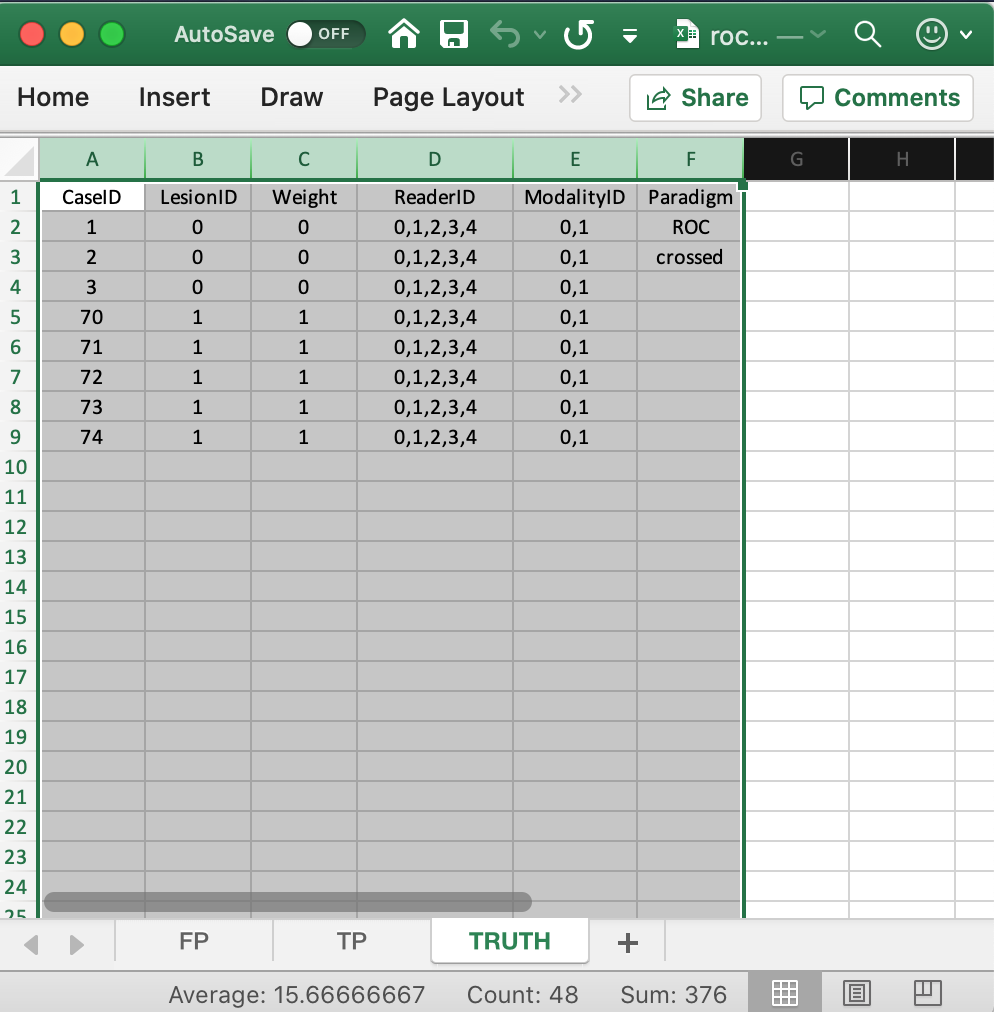
\includegraphics[width=0.5\linewidth,height=0.2\textheight]{images/rocCrTruth} 

}

\caption{Truth worksheet for file rocCr.xlsx}\label{fig:showRocCrTruthSheet}
\end{figure}

\hypertarget{the-structure-of-an-roc-dataset}{%
\section{The structure of an ROC dataset}\label{the-structure-of-an-roc-dataset}}

In the following code chunk the first statement retrieves the name of the data file, located in a hidden directory that one need not be concerned with. The second statement reads the file using the function \texttt{DfReadDataFile()} and saves it to object \texttt{x}. The third statement shows the structure of the dataset object \texttt{x}.

\begin{Shaded}
\begin{Highlighting}[]
\NormalTok{rocCr \textless{}{-}}\StringTok{ }\KeywordTok{system.file}\NormalTok{(}\StringTok{"extdata"}\NormalTok{, }\StringTok{"toyFiles/ROC/rocCr.xlsx"}\NormalTok{,}
                        \DataTypeTok{package =} \StringTok{"RJafroc"}\NormalTok{, }\DataTypeTok{mustWork =} \OtherTok{TRUE}\NormalTok{)}
\NormalTok{x \textless{}{-}}\StringTok{ }\KeywordTok{DfReadDataFile}\NormalTok{(rocCr, }\DataTypeTok{newExcelFileFormat =} \OtherTok{TRUE}\NormalTok{)}
\KeywordTok{str}\NormalTok{(x)}
\CommentTok{\#\textgreater{} List of 12}
\CommentTok{\#\textgreater{}  $ NL           : num [1:2, 1:5, 1:8, 1] 1 3 2 3 2 2 1 2 3 2 ...}
\CommentTok{\#\textgreater{}  $ LL           : num [1:2, 1:5, 1:5, 1] 5 5 5 5 5 5 5 5 5 5 ...}
\CommentTok{\#\textgreater{}  $ lesionVector : int [1:5] 1 1 1 1 1}
\CommentTok{\#\textgreater{}  $ lesionID     : num [1:5, 1] 1 1 1 1 1}
\CommentTok{\#\textgreater{}  $ lesionWeight : num [1:5, 1] 1 1 1 1 1}
\CommentTok{\#\textgreater{}  $ dataType     : chr "ROC"}
\CommentTok{\#\textgreater{}  $ modalityID   : Named chr [1:2] "0" "1"}
\CommentTok{\#\textgreater{}   ..{-} attr(*, "names")= chr [1:2] "0" "1"}
\CommentTok{\#\textgreater{}  $ readerID     : Named chr [1:5] "0" "1" "2" "3" ...}
\CommentTok{\#\textgreater{}   ..{-} attr(*, "names")= chr [1:5] "0" "1" "2" "3" ...}
\CommentTok{\#\textgreater{}  $ design       : chr "CROSSED"}
\CommentTok{\#\textgreater{}  $ normalCases  : int [1:3] 1 2 3}
\CommentTok{\#\textgreater{}  $ abnormalCases: int [1:5] 70 71 72 73 74}
\CommentTok{\#\textgreater{}  $ truthTableStr: num [1:2, 1:5, 1:8, 1:2] 1 1 1 1 1 1 1 1 1 1 ...}
\end{Highlighting}
\end{Shaded}

\begin{itemize}
\tightlist
\item
  In the above code chunk flag \texttt{newExcelFileFormat} is set to \texttt{TRUE} as otherwise columns D - F in the \texttt{Truth} worksheet are ignored and the dataset is assumed to be crossed, with \texttt{dataType} automatically determined from the contents of the FP and TP worksheets.
\item
  Flag \texttt{newExcelFileFormat\ =\ FALSE} is for compatibility with older JAFROC format Excel files, which did not have these columns in the \texttt{Truth} worksheet. Its usage is deprecated.
\item
  The dataset object \texttt{x} is a \texttt{list} variable with 12 members.
\item
  The \texttt{x\$NL} member, with dimension {[}2, 5, 8, 1{]}, contains the ratings of normal cases. The extra values in the third dimension, filled with \texttt{NAs}, are needed for compatibility with FROC datasets, as unlike ROC, false positives are possible on diseased cases.
\item
  The \texttt{x\$LL}, with dimension {[}2, 5, 5, 1{]}, contains the ratings of abnormal cases.
\item
  The \texttt{x\$lesionVector} member is a vector with 5 ones representing the 5 diseased cases in the dataset.
\item
  The \texttt{x\$lesionID} member is an array with 5 ones.
\item
  The \texttt{x\$lesionWeight} member is an array with 5 ones.
\item
  The \texttt{lesionVector}, \texttt{lesionID} and \texttt{lesionWeight} members are not used for ROC datasets. They are there for compatibility with FROC datasets.
\item
  The \texttt{dataType} member indicates that this is an \texttt{ROC} dataset.
\item
  The \texttt{x\$modalityID} member is a vector with two elements \texttt{"0"} and \texttt{"1"}, naming the two modalities.
\item
  The \texttt{x\$readerID} member is a vector with five elements \texttt{"0"}, \texttt{"1"}, \texttt{"2"}, \texttt{"3"} and \texttt{"4"}, naming the five readers.
\item
  The \texttt{x\$design} member is CROSSED; specifies the dataset design, which is ``CROSSED''.
\item
  The \texttt{x\$normalCases} member lists the integer names of the normal cases, 1, 2, 3.
\item
  The \texttt{x\$abnormalCases} member lists the integer names of the abnormal cases, 70, 71, 72, 73, 74.
\item
  The \texttt{x\$truthTableStr} member quantifies the structure of the dataset, as explained in \textbf{Chapter 00 Vignette \#3-\#5}.
\end{itemize}

\hypertarget{the-false-positive-fp-ratings}{%
\section{The false positive (FP) ratings}\label{the-false-positive-fp-ratings}}

These are found in the \texttt{FP} or \texttt{NL} worksheet, see below.

\begin{figure}

{\centering 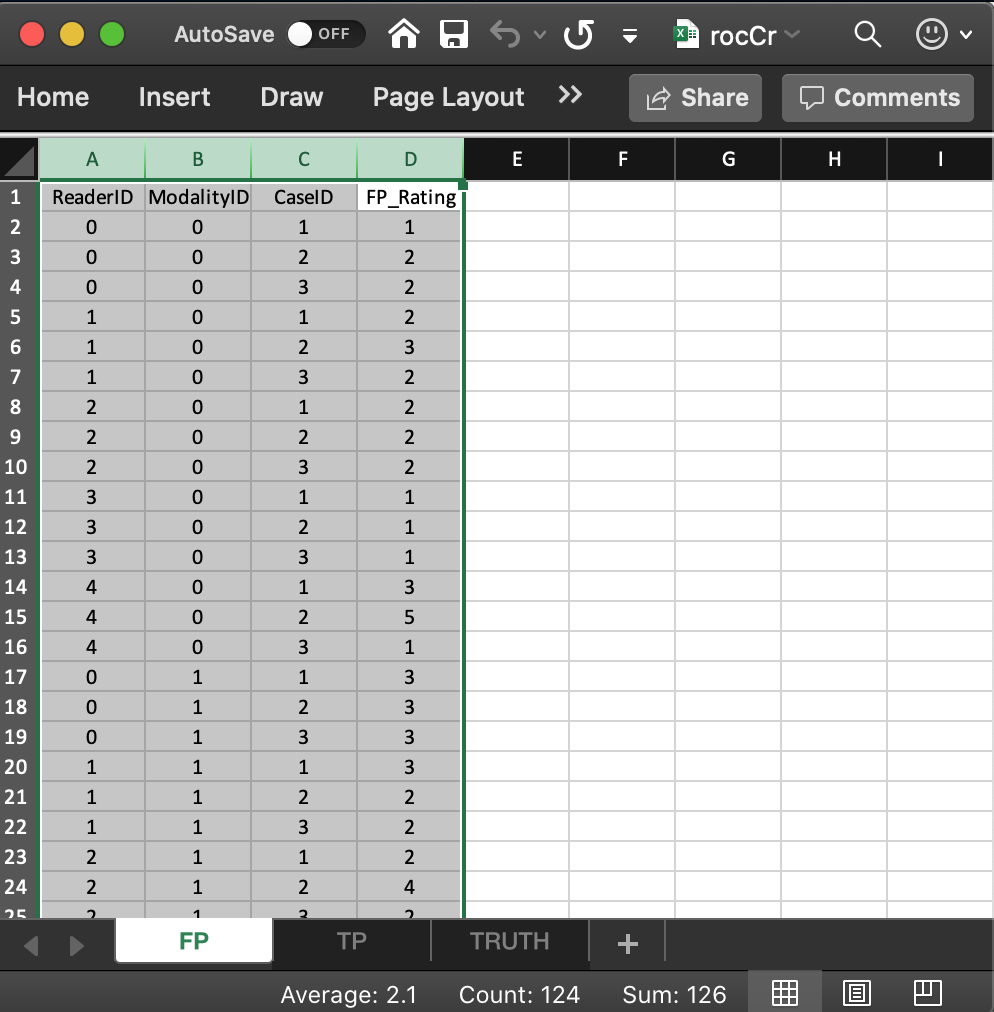
\includegraphics[width=0.5\linewidth,height=0.2\textheight]{images/rocCrFp} 

}

\caption{FP worksheet for file rocCr.xlsx}\label{fig:showRocCrFpSheet}
\end{figure}

\begin{itemize}
\tightlist
\item
  It consists of 4 columns, each of length 30 (= \# of modalities times number of readers times number of non-diseased cases).
\item
  \texttt{ReaderID}: the reader labels: \texttt{0}, \texttt{1}, \texttt{2}, \texttt{3} and \texttt{4}. Each reader label occurs 6 times (= \# of modalities times number of non-diseased cases).
\item
  \texttt{ModalityID}: the modality or treatment labels: \texttt{0} and \texttt{1}. Each label occurs 15 times (= \# of readers times number of non-diseased cases).
\item
  \texttt{CaseID}: the case labels for non-diseased cases: \texttt{1}, \texttt{2} and \texttt{3}. Each label occurs 10 times (= \# of modalities times \# of readers).
\item
  The label of a diseased case cannot occur in the FP worksheet. If it does the software generates an error.
\item
  \texttt{FP\_Rating}: the floating point ratings of non-diseased cases. Each row of this worksheet contains a rating corresponding to the values of \texttt{ReaderID}, \texttt{ModalityID} and \texttt{CaseID} for that row.
\end{itemize}

\hypertarget{the-true-positive-tp-ratings}{%
\section{The true positive (TP) ratings}\label{the-true-positive-tp-ratings}}

These are found in the \texttt{TP} or \texttt{LL} worksheet, see below.

\begin{figure}

{\centering 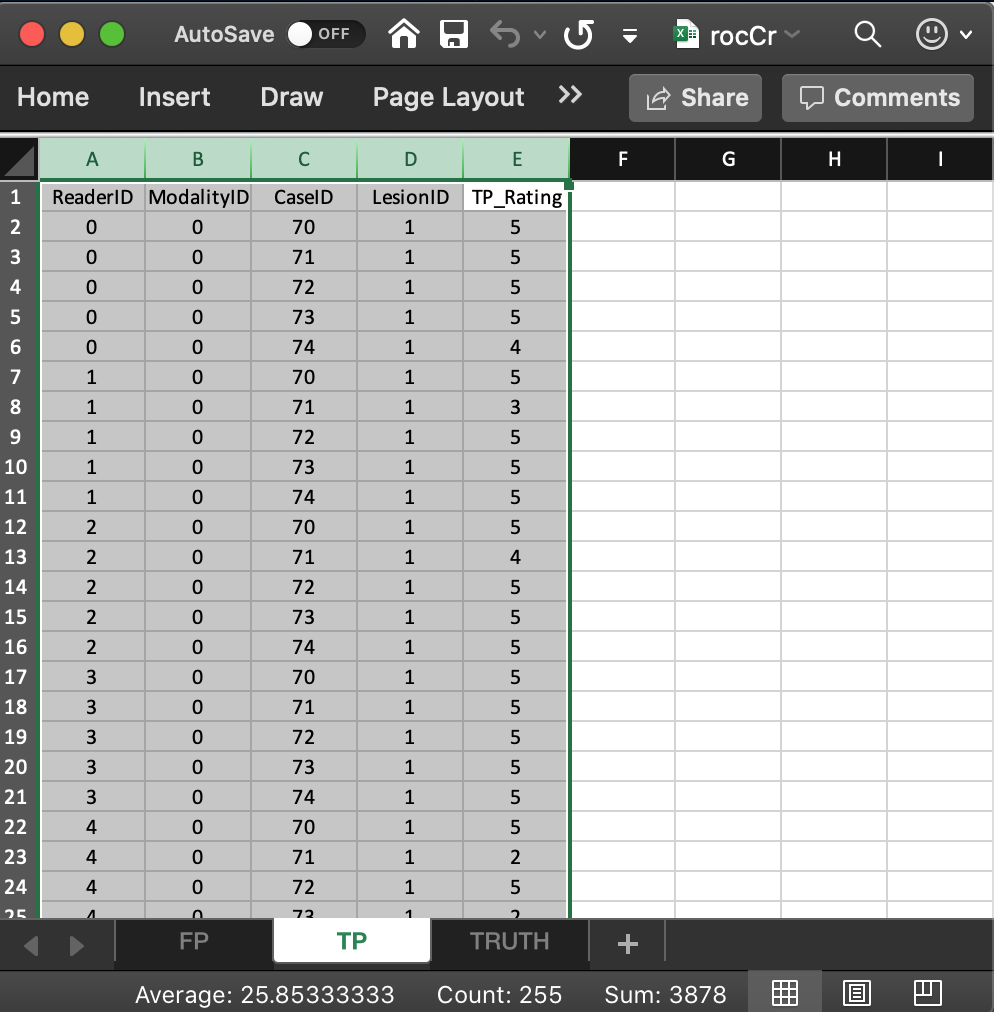
\includegraphics[width=0.5\linewidth,height=0.2\textheight]{images/rocCrTp} 

}

\caption{TP worksheet for file rocCr.xlsx}\label{fig:showRocCrTpSheet}
\end{figure}

\begin{itemize}
\tightlist
\item
  It consists of 5 columns, each of length 50 (= \# of modalities times number of readers times number of diseased cases).
\item
  \texttt{ReaderID}: the reader labels: \texttt{0}, \texttt{1}, \texttt{2}, \texttt{3} and \texttt{4}. Each reader label occurs 10 times (= \# of modalities times number of diseased cases).
\item
  \texttt{ModalityID}: the modality or treatment labels: \texttt{0} and \texttt{1}. Each label occurs 25 times (= \# of readers times number of diseased cases).
\item
  \texttt{LesionID}: For an ROC dataset this column contains fifty 1's (each diseased case has one lesion).
\item
  \texttt{CaseID}: the case labels for non-diseased cases: \texttt{70}, \texttt{71}, \texttt{72}, \texttt{73} and \texttt{74}. Each label occurs 10 times (= \# of modalities times \# of readers). The label of a non-diseased case cannot occur in the TP worksheet.
\item
  \texttt{TP\_Rating}: the floating point ratings of diseased cases. Each row of this worksheet contains a rating corresponding to the values of \texttt{ReaderID}, \texttt{ModalityID}, \texttt{LesionID} and \texttt{CaseID} for that row.
\end{itemize}

\hypertarget{correspondence-between-nl-member-of-dataset-and-the-fp-worksheet}{%
\section{\texorpdfstring{Correspondence between \texttt{NL} member of dataset and the \texttt{FP} worksheet}{Correspondence between NL member of dataset and the FP worksheet}}\label{correspondence-between-nl-member-of-dataset-and-the-fp-worksheet}}

\begin{itemize}
\tightlist
\item
  The list member \texttt{x\$NL} is an array with \texttt{dim\ =\ c(2,5,8,1)}.

  \begin{itemize}
  \tightlist
  \item
    The first dimension (2) comes from the number of modalities.
  \item
    The second dimension (5) comes from the number of readers.
  \item
    The third dimension (8) comes from the \textbf{total} number of cases.
  \item
    The fourth dimension is alway 1 for an ROC dataset.
  \end{itemize}
\item
  The value of \texttt{x\$NL{[}1,5,2,1{]}}, i.e., 5, corresponds to row 15 of the FP table, i.e., to \texttt{ModalityID} = 0, \texttt{ReaderID} = 4 and \texttt{CaseID} = 2.
\item
  The value of \texttt{x\$NL{[}2,3,2,1{]}}, i.e., 4, corresponds to row 24 of the FP table, i.e., to \texttt{ModalityID} 1, \texttt{ReaderID} 2 and \texttt{CaseID} 2.
\item
  All values for case index \textgreater{} 3 are \texttt{-Inf}. For example the value of \texttt{x\$NL{[}2,3,4,1{]}} is \texttt{-Inf}. This is because there are only 3 non-diseased cases. The extra length is needed for compatibility with FROC datasets.
\end{itemize}

\hypertarget{correspondence-between-ll-member-of-dataset-and-the-tp-worksheet}{%
\section{\texorpdfstring{Correspondence between \texttt{LL} member of dataset and the \texttt{TP} worksheet}{Correspondence between LL member of dataset and the TP worksheet}}\label{correspondence-between-ll-member-of-dataset-and-the-tp-worksheet}}

\begin{itemize}
\tightlist
\item
  The list member \texttt{x\$LL} is an array with \texttt{dim\ =\ c(2,5,5,1)}.

  \begin{itemize}
  \tightlist
  \item
    The first dimension (2) comes from the number of modalities.
  \item
    The second dimension (5) comes from the number of readers.
  \item
    The third dimension (5) comes from the number of diseased cases.
  \item
    The fourth dimension is alway 1 for an ROC dataset.
  \end{itemize}
\item
  The value of \texttt{x\$LL{[}1,1,5,1{]}}, i.e., 4, corresponds to row 6 of the TP table, i.e., to \texttt{ModalityID} = 0, \texttt{ReaderID} = 0 and \texttt{CaseID} = 74.
\item
  The value of \texttt{x\$LL{[}1,2,2,1{]}}, i.e., 3, corresponds to row 8 of the TP table, i.e., to \texttt{ModalityID} = 0, \texttt{ReaderID} = 1 and \texttt{CaseID} = 71.
\item
  There are no -Inf values in \texttt{x\$LL}: \texttt{any(x\$LL\ ==\ -Inf)} = FALSE.
\end{itemize}

\hypertarget{correspondence-using-the-which-function}{%
\section{\texorpdfstring{Correspondence using the \texttt{which} function}{Correspondence using the which function}}\label{correspondence-using-the-which-function}}

\begin{itemize}
\tightlist
\item
  Converting from \textbf{names} to \textbf{subscripts} (indicating position in an array) can be confusing.
\item
  The following example uses the \texttt{which} function to help out.
\item
  The first line says that the \texttt{abnormalCase} named 70 corresponds to subscript 1 in the LL array case dimension.
\item
  The second line prints the NL rating for \texttt{modalityID} = 0, \texttt{readerID} = 1 and \texttt{normalCases} = 1.
\item
  The third line prints the LL rating for \texttt{modalityID} = 0, \texttt{readerID} = 1 and \texttt{abnormalCases} = 70.
\item
  The last line shows what happens if one enters an invalid value for name; the result is a \texttt{numeric(0)}.
\item
  Note that in each of these examples, the last dimension is 1 because we are dealing with an ROC dataset.
\item
  The reader is encouraged to examine the correspondence between the NL and LL ratings and the Excel file using this method.
\end{itemize}

\begin{Shaded}
\begin{Highlighting}[]
\KeywordTok{which}\NormalTok{(x}\OperatorTok{$}\NormalTok{abnormalCases }\OperatorTok{==}\StringTok{ }\DecValTok{70}\NormalTok{)}
\CommentTok{\#\textgreater{} [1] 1}
\NormalTok{x}\OperatorTok{$}\NormalTok{NL[}\KeywordTok{which}\NormalTok{(x}\OperatorTok{$}\NormalTok{modalityID }\OperatorTok{==}\StringTok{ "0"}\NormalTok{),}\KeywordTok{which}\NormalTok{(x}\OperatorTok{$}\NormalTok{readerID }\OperatorTok{==}\StringTok{ "1"}\NormalTok{),}\KeywordTok{which}\NormalTok{(x}\OperatorTok{$}\NormalTok{normalCases }\OperatorTok{==}\StringTok{ }\DecValTok{1}\NormalTok{),}\DecValTok{1}\NormalTok{]}
\CommentTok{\#\textgreater{} [1] 2}
\NormalTok{x}\OperatorTok{$}\NormalTok{LL[}\KeywordTok{which}\NormalTok{(x}\OperatorTok{$}\NormalTok{modalityID }\OperatorTok{==}\StringTok{ "0"}\NormalTok{),}\KeywordTok{which}\NormalTok{(x}\OperatorTok{$}\NormalTok{readerID }\OperatorTok{==}\StringTok{ "1"}\NormalTok{),}\KeywordTok{which}\NormalTok{(x}\OperatorTok{$}\NormalTok{abnormalCases }\OperatorTok{==}\StringTok{ }\DecValTok{70}\NormalTok{),}\DecValTok{1}\NormalTok{]}
\CommentTok{\#\textgreater{} [1] 5}
\NormalTok{x}\OperatorTok{$}\NormalTok{LL[}\KeywordTok{which}\NormalTok{(x}\OperatorTok{$}\NormalTok{modalityID }\OperatorTok{==}\StringTok{ "a"}\NormalTok{),}\KeywordTok{which}\NormalTok{(x}\OperatorTok{$}\NormalTok{readerID }\OperatorTok{==}\StringTok{ "1"}\NormalTok{),}\KeywordTok{which}\NormalTok{(x}\OperatorTok{$}\NormalTok{abnormalCases }\OperatorTok{==}\StringTok{ }\DecValTok{70}\NormalTok{),}\DecValTok{1}\NormalTok{]}
\CommentTok{\#\textgreater{} numeric(0)}
\end{Highlighting}
\end{Shaded}

\hypertarget{references-1}{%
\section{References}\label{references-1}}

\hypertarget{SSFDistr}{%
\chapter{BACKGROUND ON THE F-DISTRIBUTION}\label{SSFDistr}}

\hypertarget{introduction-1}{%
\section{Introduction}\label{introduction-1}}

Since it plays an important role in sample size estimation, it is helpful to examine the behavior of the F-distribution. In the following \texttt{ndf} = numerator degrees of freedom, \texttt{ddf} = denominator degrees of freedom and \texttt{ncp} = non-centrality parameter (i.e., the \(\Delta\) appearing in Eqn. (11.6) of \citep{RN2680}).

The use of three \texttt{R} functions is demonstrated.

\begin{itemize}
\item
  \texttt{qf(p,ndf,ddf)} is the \emph{quantile} function of the F-distribution for specified values of \texttt{p}, \texttt{ndf} and \texttt{ddf}, i.e., the value \texttt{x} such that fraction \texttt{p} of the area under the F-distribution lies to the right of \texttt{x}. Since \texttt{ncp} is not included as a parameter, the default value, i.e., zero, is used. This is called the \emph{central} F-distribution.
\item
  \texttt{df(x,ndf,ddf,ncp)} is the probability density function (\emph{pdf}) of the F-distribution, as a function of \texttt{x}, for specified values of \texttt{ndf}, \texttt{ddf} and \texttt{ncp}.
\item
  \texttt{pf(x,ndf,ddf,ncp)} is the probability (or cumulative) distribution function of the F-distribution for specified values of \texttt{ndf}, \texttt{ddf} and \texttt{ncp}.
\end{itemize}

\hypertarget{effect-of-ncp-for-ndf-2-and-ddf-10}{%
\section{\texorpdfstring{Effect of \texttt{ncp} for \texttt{ndf} = 2 and \texttt{ddf} = 10}{Effect of ncp for ndf = 2 and ddf = 10}}\label{effect-of-ncp-for-ndf-2-and-ddf-10}}

\begin{itemize}
\tightlist
\item
  Four values of \texttt{ncp} are considered (0, 2, 5, 10) for \texttt{ddf} = 10.
\item
  \texttt{fCrit} is the critical value of the F distribution, i.e., that value such that fraction \(\alpha\) of the area is to the right of the critical value, i.e., \texttt{fCrit} is identical to:
  \begin{equation*} 
  F_{1-\alpha ,ndf,ddf}
  \end{equation*}
\end{itemize}

\begin{Shaded}
\begin{Highlighting}[]
\NormalTok{ndf \textless{}{-}}\StringTok{ }\DecValTok{2}\NormalTok{;ddf \textless{}{-}}\StringTok{ }\DecValTok{10}\NormalTok{;ncp \textless{}{-}}\StringTok{ }\KeywordTok{c}\NormalTok{(}\DecValTok{0}\NormalTok{,}\DecValTok{2}\NormalTok{,}\DecValTok{5}\NormalTok{,}\DecValTok{10}\NormalTok{)}
\NormalTok{alpha \textless{}{-}}\StringTok{ }\FloatTok{0.05}
\NormalTok{fCrit \textless{}{-}}\StringTok{ }\KeywordTok{qf}\NormalTok{(}\DecValTok{1}\OperatorTok{{-}}\NormalTok{alpha, ndf,ddf)}
\NormalTok{x \textless{}{-}}\StringTok{ }\KeywordTok{seq}\NormalTok{(}\DecValTok{1}\NormalTok{, }\DecValTok{20}\NormalTok{, }\FloatTok{0.1}\NormalTok{)}
\NormalTok{myLabel \textless{}{-}}\StringTok{ }\KeywordTok{c}\NormalTok{(}\StringTok{"A"}\NormalTok{, }\StringTok{"B"}\NormalTok{, }\StringTok{"C"}\NormalTok{, }\StringTok{"D"}\NormalTok{)}
\NormalTok{myLabelIndx \textless{}{-}}\StringTok{ }\DecValTok{1}
\NormalTok{pFgtFCrit \textless{}{-}}\StringTok{ }\OtherTok{NULL}
\ControlFlowTok{for}\NormalTok{ (i }\ControlFlowTok{in} \DecValTok{1}\OperatorTok{:}\KeywordTok{length}\NormalTok{(ncp))}
\NormalTok{\{}
\NormalTok{  y \textless{}{-}}\StringTok{ }\KeywordTok{df}\NormalTok{(x,ndf,ddf,}\DataTypeTok{ncp=}\NormalTok{ncp[i])}
\NormalTok{  pFgtFCrit \textless{}{-}}\StringTok{ }\KeywordTok{c}\NormalTok{(pFgtFCrit, }\DecValTok{1}\OperatorTok{{-}}\KeywordTok{pf}\NormalTok{(fCrit, ndf, ddf, }\DataTypeTok{ncp =}\NormalTok{ ncp[i]))}
\NormalTok{\}  }
\ControlFlowTok{for}\NormalTok{ (i }\ControlFlowTok{in} \DecValTok{1}\OperatorTok{:}\KeywordTok{length}\NormalTok{(ncp))}
\NormalTok{\{}
\NormalTok{  y \textless{}{-}}\StringTok{ }\KeywordTok{df}\NormalTok{(x,ndf,ddf,}\DataTypeTok{ncp=}\NormalTok{ncp[i])}
\NormalTok{  curveData \textless{}{-}}\StringTok{ }\KeywordTok{data.frame}\NormalTok{(}\DataTypeTok{x =}\NormalTok{ x, }\DataTypeTok{pdf =}\NormalTok{ y)}
\NormalTok{  curvePlot \textless{}{-}}\StringTok{ }\KeywordTok{ggplot}\NormalTok{(}\DataTypeTok{data =}\NormalTok{ curveData, }\DataTypeTok{mapping =} \KeywordTok{aes}\NormalTok{(}\DataTypeTok{x =}\NormalTok{ x, }\DataTypeTok{y =}\NormalTok{ pdf)) }\OperatorTok{+}\StringTok{ }
\StringTok{    }\KeywordTok{geom\_line}\NormalTok{() }\OperatorTok{+}
\StringTok{    }\KeywordTok{ggtitle}\NormalTok{(myLabel[myLabelIndx]);myLabelIndx \textless{}{-}}\StringTok{ }\NormalTok{myLabelIndx }\OperatorTok{+}\StringTok{ }\DecValTok{1}
  \KeywordTok{print}\NormalTok{(curvePlot)}
\NormalTok{\}}
\NormalTok{fCrit\_}\DecValTok{2}\NormalTok{\_}\DecValTok{10}\NormalTok{ \textless{}{-}}\StringTok{ }\NormalTok{fCrit }\CommentTok{\# convention fCrit\_ndf\_ddf}
\end{Highlighting}
\end{Shaded}

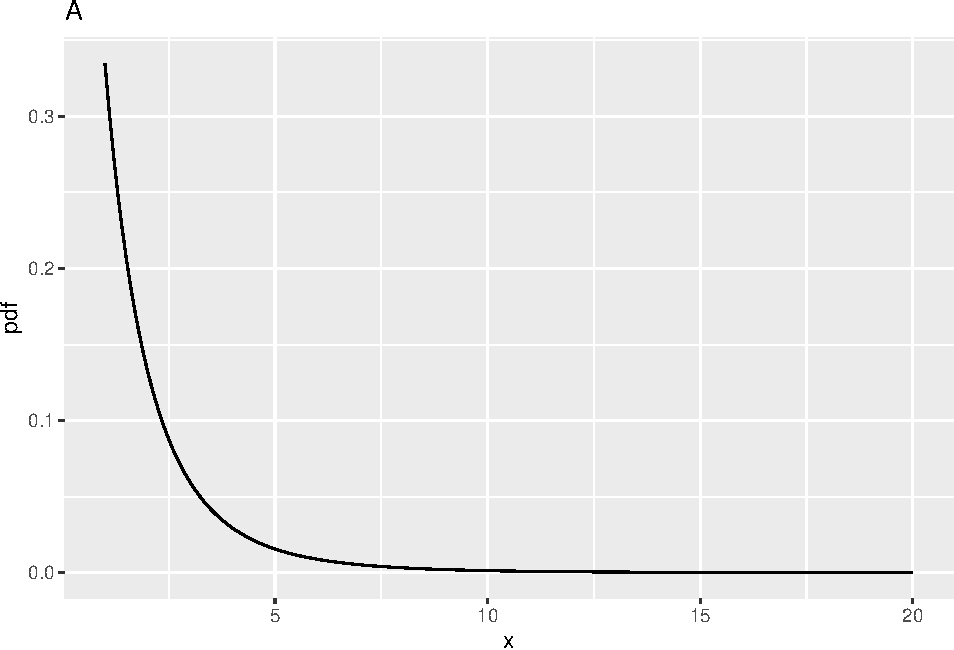
\includegraphics{11-SampleSize1_files/figure-latex/unnamed-chunk-1-1.pdf} 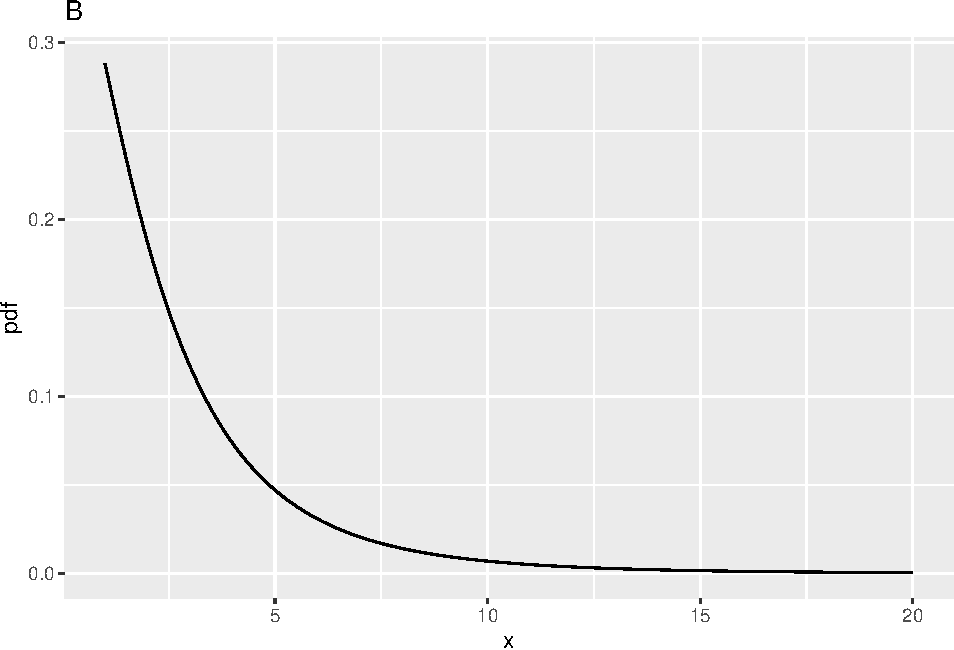
\includegraphics{11-SampleSize1_files/figure-latex/unnamed-chunk-1-2.pdf} 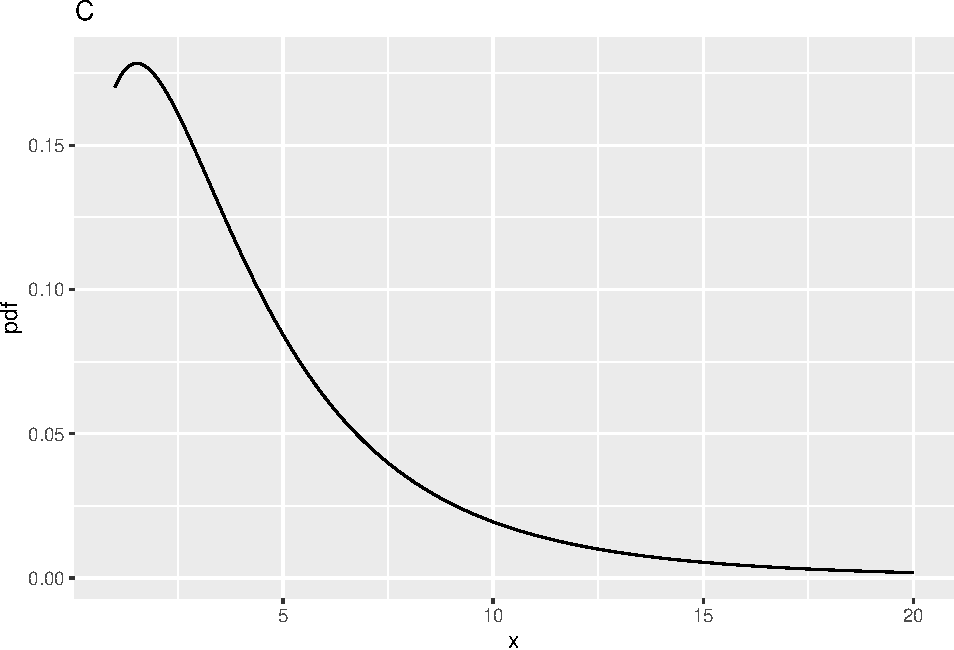
\includegraphics{11-SampleSize1_files/figure-latex/unnamed-chunk-1-3.pdf} 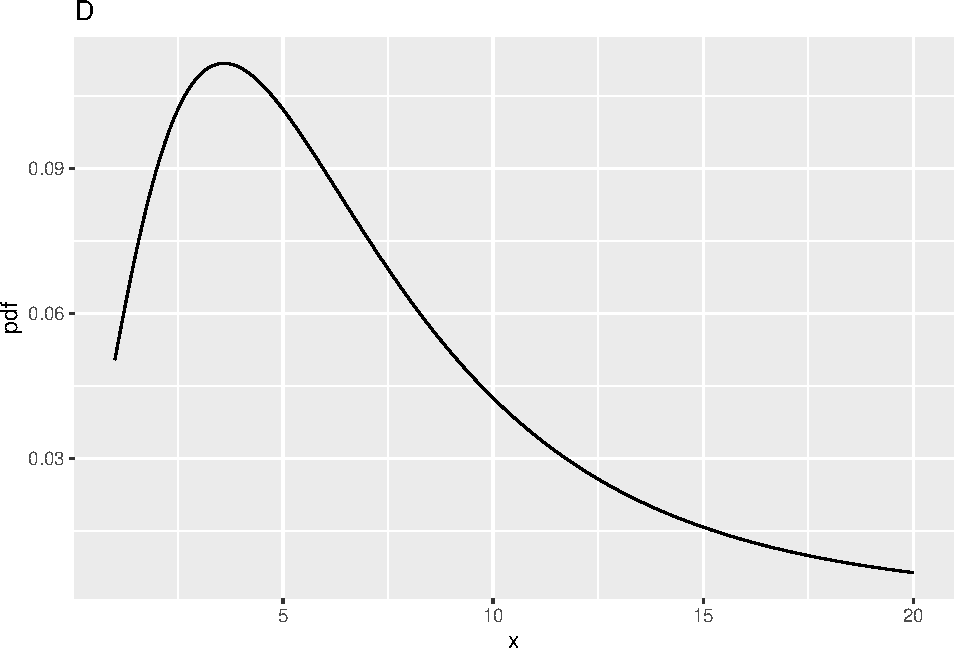
\includegraphics{11-SampleSize1_files/figure-latex/unnamed-chunk-1-4.pdf}

\begin{tabular}{l|r|r|r|r|r}
\hline
  & ndf & ddf & fCrit & ncp & pFgtFCrit\\
\hline
A & 2 & 10 & 4.102821 & 0 & 0.0500000\\
\hline
B & 2 & 10 & 4.102821 & 2 & 0.1775840\\
\hline
C & 2 & 10 & 4.102821 & 5 & 0.3876841\\
\hline
D & 2 & 10 & 4.102821 & 10 & 0.6769776\\
\hline
\end{tabular}

\hypertarget{comments}{%
\section{Comments}\label{comments}}

\hypertarget{fig.-a}{%
\subsection{Fig. A}\label{fig.-a}}

\begin{itemize}
\tightlist
\item
  This corresponds to \texttt{ncp\ =\ 0}, i.e., the \emph{central} F-distribution.
\item
  The integral under this distribution is unity (this is also true for all plots in this vignette).
\item
  The critical value, \texttt{fCrit} in the above code block, is the value of \texttt{x} such that the probability of exceeding \texttt{x} is \(\alpha\). The corresponding parameter \texttt{alpha} is defined above as 0.05.
\item
  In the current example \texttt{fCrit} = 4.102821. Notice the use of the quantile function \texttt{qf()} to determine this value, and the default value of \texttt{ncp}, namely zero, is used; specifically, one does not pass a 4th argument to \texttt{qf()}.
\item
  \textbf{The decision rule for rejecting the NH uses the NH distribution of the F-statistic}, i.e., reject the NH if F \textgreater= \texttt{fCrit}. As expected, \texttt{prob\ \textgreater{}\ fCrit} = 0.05 because this is how \texttt{fCrit} was defined.
\end{itemize}

\hypertarget{fig.-b}{%
\subsection{Fig. B}\label{fig.-b}}

\begin{itemize}
\tightlist
\item
  This corresponds to \texttt{ncp\ =\ 2}, \texttt{ndf} = 2 and \texttt{ddf} = 10.
\item
  The distribution is slightly shifted to the right as compared to Fig. A, thereby making it more likely that the observed value of the F-statistic will exceed the critical value determined for the NH distribution.
\item
  In fact, \texttt{prob\ \textgreater{}\ fCrit} = 0.177584, i.e., the \emph{statistical power} (compare this to Fig. A where \texttt{prob\ \textgreater{}\ fCrit} was 0.05).
\end{itemize}

\hypertarget{fig.-c}{%
\subsection{Fig. C}\label{fig.-c}}

\begin{itemize}
\tightlist
\item
  This corresponds to \texttt{ncp\ =\ 5}, \texttt{ndf} = 2 and \texttt{ddf} = 10.
\item
  Now \texttt{prob\ \textgreater{}\ fCrit} = 0.3876841.
\item
  Power has increased compared to Fig. B.
\end{itemize}

\hypertarget{fig.-d}{%
\subsection{Fig. D}\label{fig.-d}}

\begin{itemize}
\tightlist
\item
  This corresponds to \texttt{ncp\ =\ 10}, \texttt{ndf} = 2 and \texttt{ddf} = 10.
\item
  Now \texttt{prob\ \textgreater{}\ fCrit} is 0.6769776.
\item
  Power has increased compared to Fig. C.
\item
  The effect of the shift is most obvious in Fig. C and Fig. D.
\item
  Considering a vertical line at \texttt{x} = 4.102821, fraction 0.6769776 of the probability distribution in Fig. D lies to the right of this line
\item
  Therefore the NH is likely to be rejected with probability 0.6769776.
\end{itemize}

\hypertarget{summary}{%
\subsection{Summary}\label{summary}}

The larger that non-centrality parameter, the greater the shift to the right of the F-distribution, and the greater the statistical power.

\hypertarget{effect-of-ncp-for-ndf-2-and-ddf-100}{%
\section{\texorpdfstring{Effect of \texttt{ncp} for \texttt{ndf} = 2 and \texttt{ddf} = 100}{Effect of ncp for ndf = 2 and ddf = 100}}\label{effect-of-ncp-for-ndf-2-and-ddf-100}}

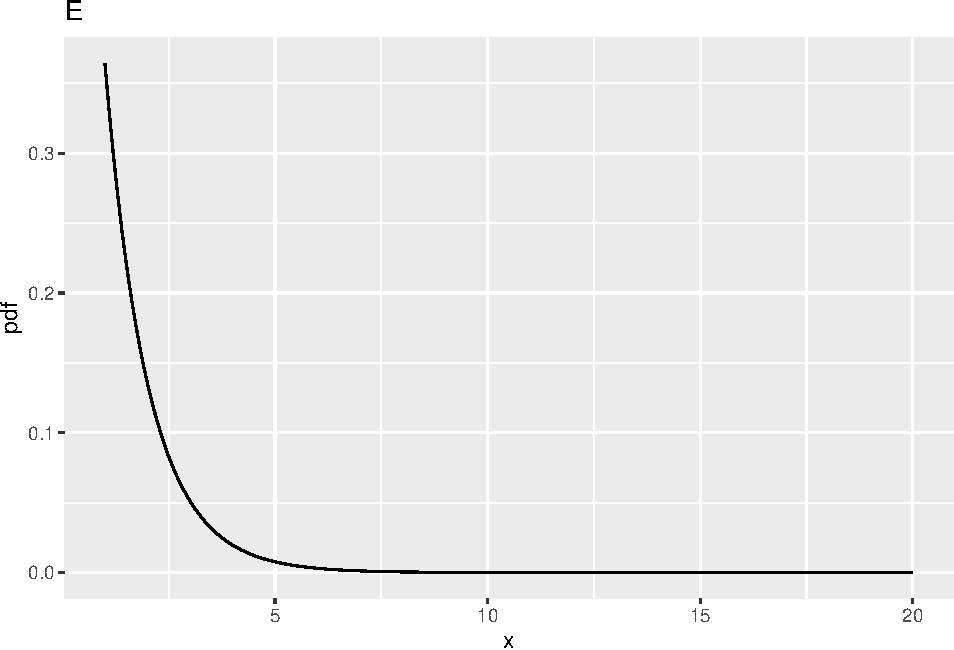
\includegraphics{11-SampleSize1_files/figure-latex/unnamed-chunk-3-1.pdf} 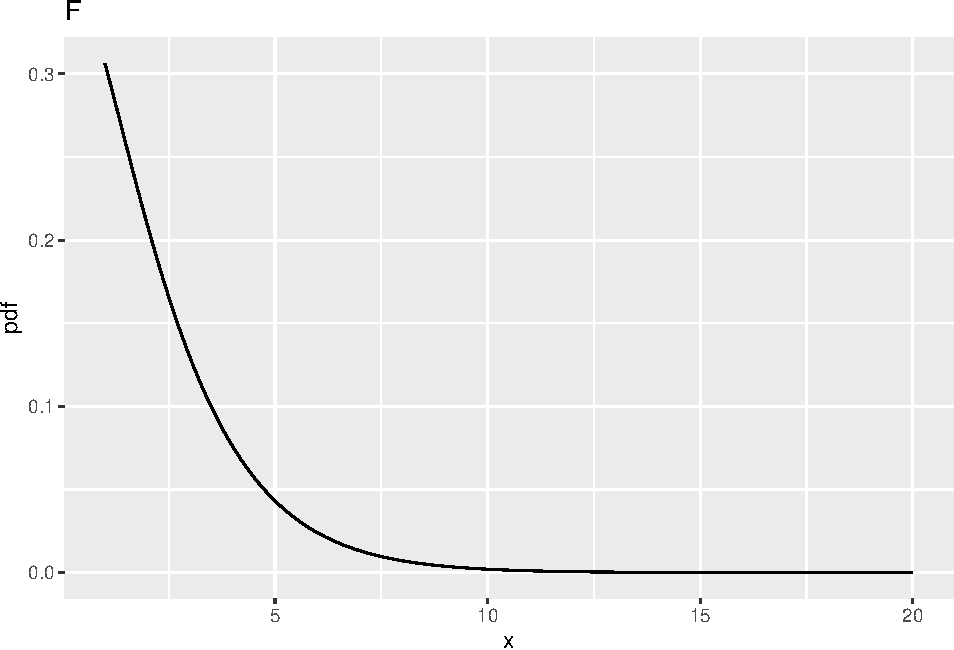
\includegraphics{11-SampleSize1_files/figure-latex/unnamed-chunk-3-2.pdf} 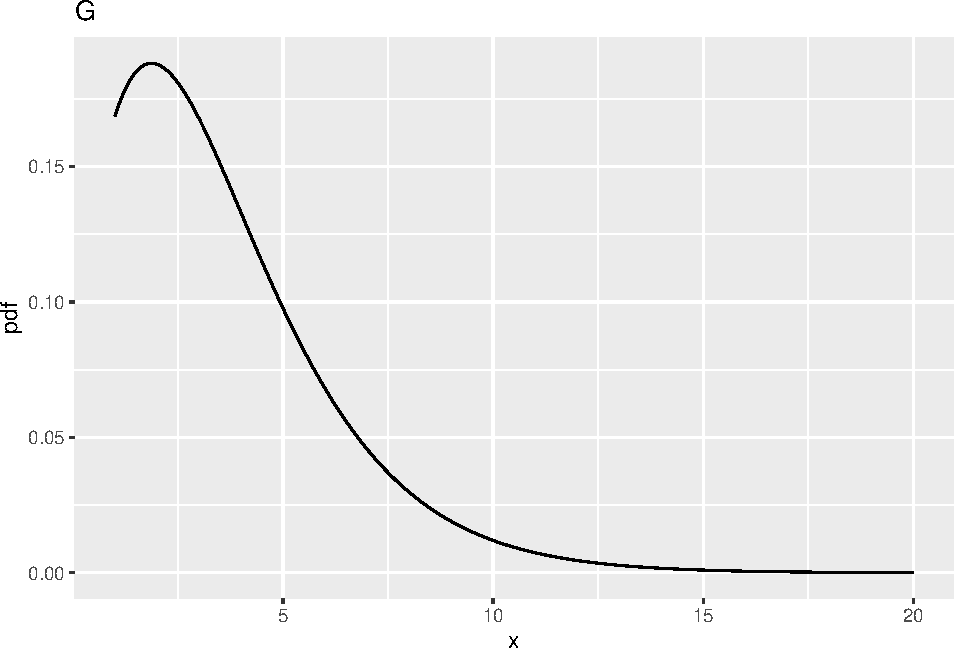
\includegraphics{11-SampleSize1_files/figure-latex/unnamed-chunk-3-3.pdf} 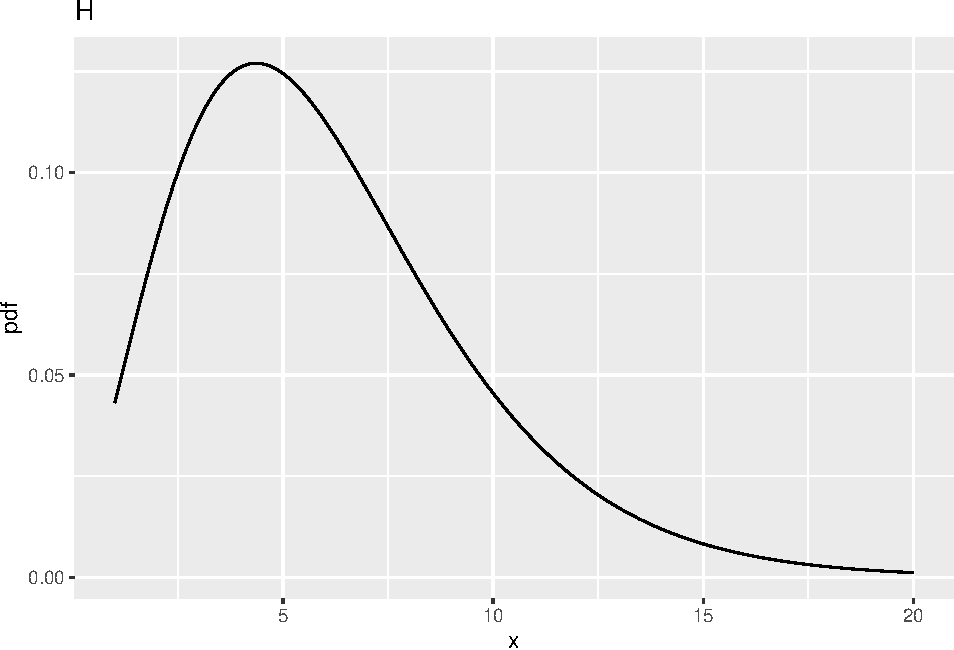
\includegraphics{11-SampleSize1_files/figure-latex/unnamed-chunk-3-4.pdf}

\begin{tabular}{l|r|r|r|r|r}
\hline
  & ndf & ddf & fCrit & ncp & pFgtFCrit\\
\hline
A & 2 & 10 & 4.102821 & 0 & 0.0500000\\
\hline
B & 2 & 10 & 4.102821 & 2 & 0.1775840\\
\hline
C & 2 & 10 & 4.102821 & 5 & 0.3876841\\
\hline
D & 2 & 10 & 4.102821 & 10 & 0.6769776\\
\hline
E & 2 & 100 & 3.087296 & 0 & 0.0500000\\
\hline
F & 2 & 100 & 3.087296 & 2 & 0.2199264\\
\hline
G & 2 & 100 & 3.087296 & 5 & 0.4910802\\
\hline
H & 2 & 100 & 3.087296 & 10 & 0.8029764\\
\hline
\end{tabular}

\hypertarget{comments-1}{%
\section{Comments}\label{comments-1}}

\begin{itemize}
\tightlist
\item
  All comparisons in this sections are at the same values of \texttt{ncp} defined above.
\item
  And between \texttt{ddf} = 100 and \texttt{ddf} = 10.
\end{itemize}

\hypertarget{fig.-e}{%
\subsection{Fig. E}\label{fig.-e}}

\begin{itemize}
\tightlist
\item
  This corresponds to \texttt{ncp} = 0, \texttt{ndf} = 2 and \texttt{ddf} = 100.
\item
  The critical value is \texttt{fCrit\_2\_100} = 3.0872959. Notice the decrease compared to the previous value for \texttt{ncp} = 0, i.e., 4.102821, for \texttt{ddf} = 10.
\item
  One expects that increasing \texttt{ddf} will make it more likely that the NH will be rejected, and this is confirmed below.
\item
  All else equal, statistical power increases with increasing \texttt{ddf}.
\end{itemize}

\hypertarget{fig.-f}{%
\subsection{Fig. F}\label{fig.-f}}

\begin{itemize}
\tightlist
\item
  This corresponds to \texttt{ncp} = 2, \texttt{ndf} = 2 and \texttt{ddf} = 100.
\item
  The probability of exceeding the critical value is \texttt{prob\ \textgreater{}\ fCrit\_2\_100} = 0.2199264, greater than the previous value, i.e., 0.177584 for \texttt{ddf} = 10.
\end{itemize}

\hypertarget{fig.-g}{%
\subsection{Fig. G}\label{fig.-g}}

\begin{itemize}
\tightlist
\item
  This corresponds to \texttt{ncp\ =\ 5}, \texttt{ndf} = 2 and \texttt{ddf} = 100.
\item
  The probability of exceeding the critical value is \texttt{prob\ \textgreater{}\ fCrit\_2\_100} = 0.4910802.
\item
  This is greater than the previous value, i.e., 0.3876841 for \texttt{ddf} = 10.
\end{itemize}

\hypertarget{fig.-h}{%
\subsection{Fig. H}\label{fig.-h}}

\begin{itemize}
\tightlist
\item
  This corresponds to \texttt{ncp\ =\ 10}, \texttt{ndf} = 2 and \texttt{ddf} = 100.
\item
  The probability of exceeding the critical value is \texttt{prob\ \textgreater{}\ fCrit\_2\_100} is 0.8029764.
\item
  This is greater than the previous value, i.e., 0.6769776 for \texttt{ddf} = 10.
\end{itemize}

\hypertarget{effect-of-ncp-for-ndf-1-ddf-100}{%
\section{\texorpdfstring{Effect of \texttt{ncp} for \texttt{ndf} = 1, \texttt{ddf} = 100}{Effect of ncp for ndf = 1, ddf = 100}}\label{effect-of-ncp-for-ndf-1-ddf-100}}

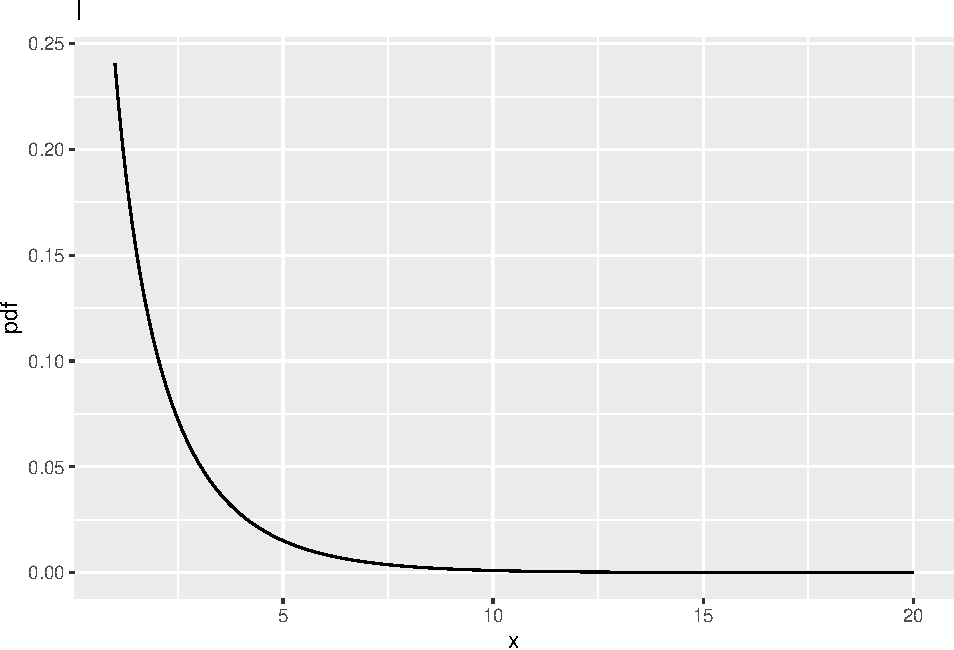
\includegraphics{11-SampleSize1_files/figure-latex/unnamed-chunk-5-1.pdf} 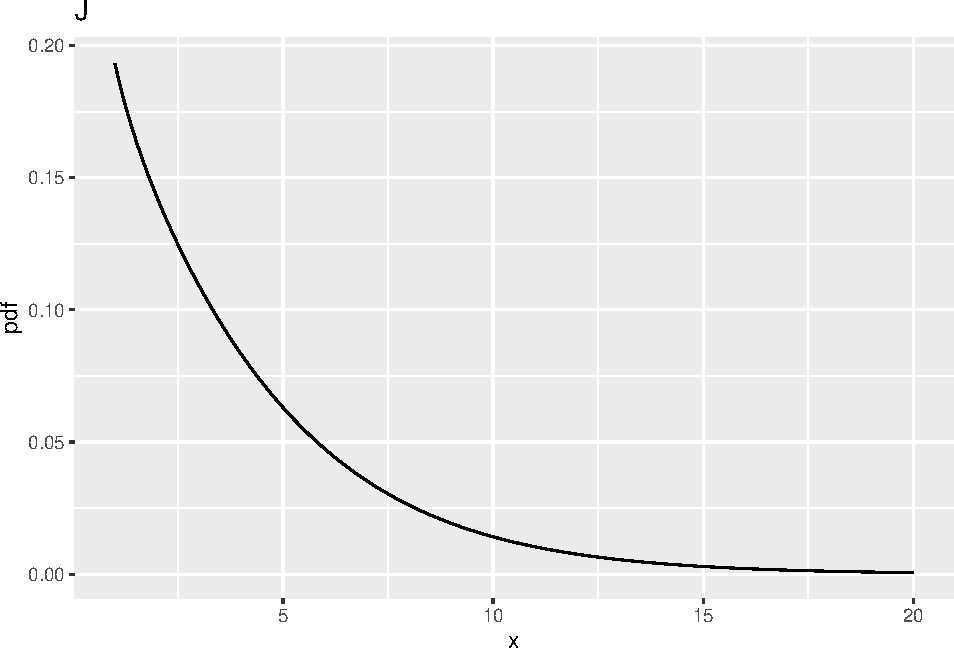
\includegraphics{11-SampleSize1_files/figure-latex/unnamed-chunk-5-2.pdf} 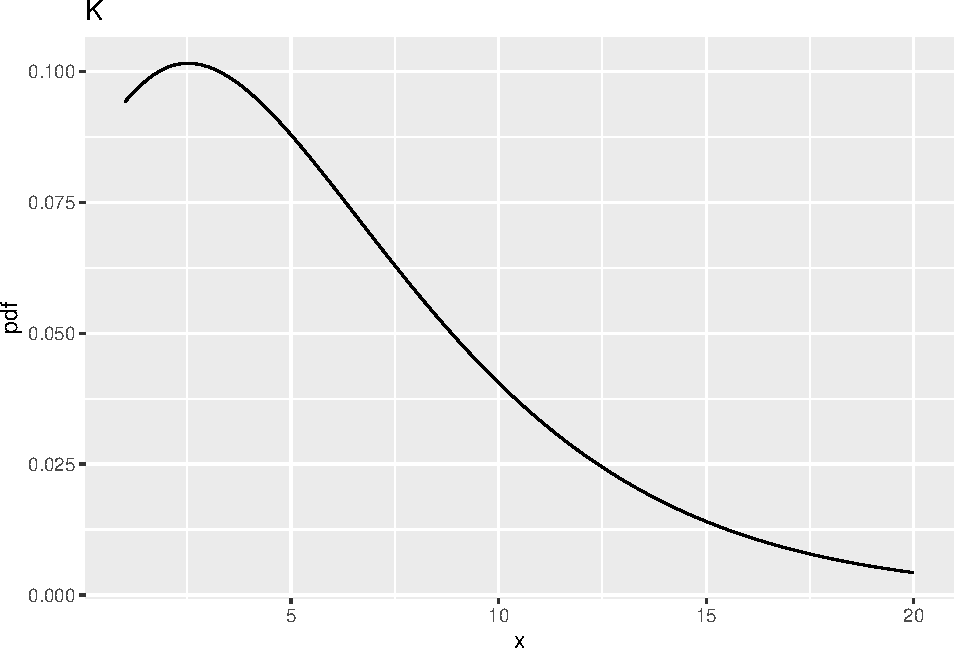
\includegraphics{11-SampleSize1_files/figure-latex/unnamed-chunk-5-3.pdf} 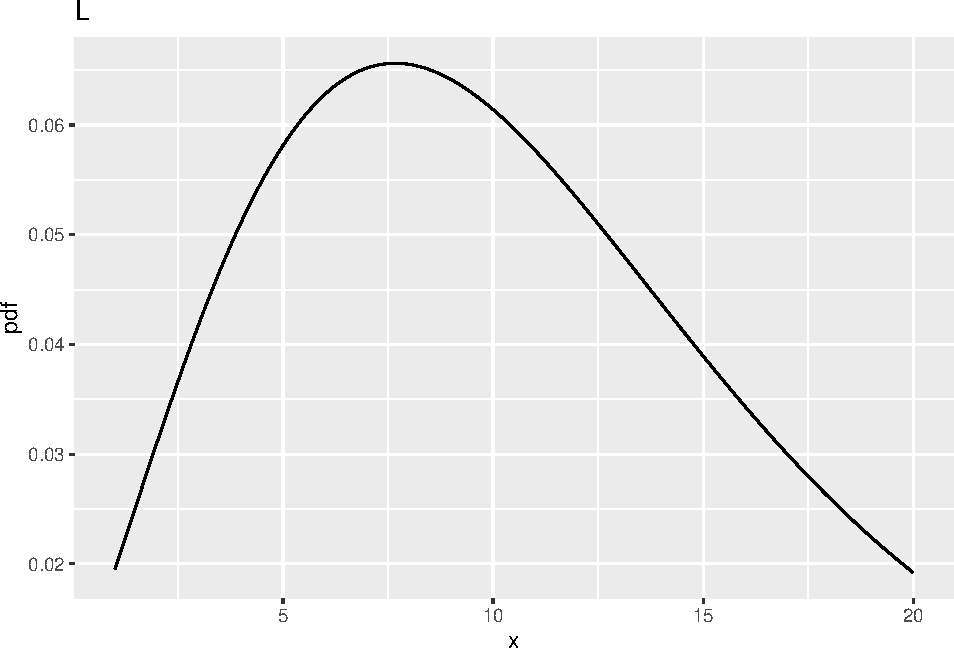
\includegraphics{11-SampleSize1_files/figure-latex/unnamed-chunk-5-4.pdf}

\begin{tabular}{l|r|r|r|r|r}
\hline
  & ndf & ddf & fCrit & ncp & pFgtFCrit\\
\hline
A & 2 & 10 & 4.102821 & 0 & 0.0500000\\
\hline
B & 2 & 10 & 4.102821 & 2 & 0.1775840\\
\hline
C & 2 & 10 & 4.102821 & 5 & 0.3876841\\
\hline
D & 2 & 10 & 4.102821 & 10 & 0.6769776\\
\hline
E & 2 & 100 & 3.087296 & 0 & 0.0500000\\
\hline
F & 2 & 100 & 3.087296 & 2 & 0.2199264\\
\hline
G & 2 & 100 & 3.087296 & 5 & 0.4910802\\
\hline
H & 2 & 100 & 3.087296 & 10 & 0.8029764\\
\hline
I & 1 & 100 & 3.936143 & 0 & 0.0500000\\
\hline
J & 1 & 100 & 3.936143 & 2 & 0.2883607\\
\hline
K & 1 & 100 & 3.936143 & 5 & 0.6004962\\
\hline
L & 1 & 100 & 3.936143 & 10 & 0.8793619\\
\hline
\end{tabular}

\hypertarget{comments-2}{%
\section{Comments}\label{comments-2}}

\begin{itemize}
\tightlist
\item
  All comparisons in this sections are at the same values of \texttt{ncp} defined above and at \texttt{ddf} = 100.
\item
  And between \texttt{ndf} = 1 and \texttt{ndf} = 2.
\end{itemize}

\hypertarget{fig.-i}{%
\subsection{Fig. I}\label{fig.-i}}

\begin{itemize}
\tightlist
\item
  This corresponds to \texttt{ncp} = 0, \texttt{ndf} = 1 and \texttt{ddf} = 100.
\item
  The critical value is \texttt{fCrit\_1\_100} = 3.936143.
\item
  Notice the increase in the critical value as compared to the corresponding value for \texttt{ndf\ =\ 2}, i.e., 3.0872959.
\item
  One might expect power to decrease, \textbf{but see below}.
\end{itemize}

\hypertarget{fig.-j}{%
\subsection{Fig. J}\label{fig.-j}}

\begin{itemize}
\tightlist
\item
  This corresponds to \texttt{ncp} = 2, \texttt{ndf} = 1 and \texttt{ddf} = 100.
\item
  Now \texttt{prob\ \textgreater{}\ fCrit\_1\_100} = 0.2883607, larger than the previous value 0.2199264.
\item
  The power has actually increased.
\end{itemize}

\hypertarget{fig.-k}{%
\subsection{Fig. K}\label{fig.-k}}

\begin{itemize}
\tightlist
\item
  This corresponds to \texttt{ncp} = 5, \texttt{ndf} = 1 and \texttt{ddf} = 100`',
\item
  Now \texttt{prob\ \textgreater{}\ fCrit\_1\_100} = 0.6004962, larger than the previous value 0.4910802.
\item
  Again, the power has actually increased.
\end{itemize}

\hypertarget{fig.-l}{%
\subsection{Fig. L}\label{fig.-l}}

\begin{itemize}
\tightlist
\item
  This corresponds to \texttt{ncp} = 10, \texttt{ndf} = 1 and \texttt{ddf} = 100
\item
  Now \texttt{prob\ \textgreater{}\ fCrit\_1\_100} is 0.8793619, larger than the previous value 0.8029764.
\item
  The power has actually increased.
\end{itemize}

\hypertarget{summary-1}{%
\section{Summary}\label{summary-1}}

\begin{itemize}
\tightlist
\item
  Power increases with increasing \texttt{ddf} and \texttt{ncp}.
\item
  The effect of increasing \texttt{ncp} is quite dramatic. This is because power depends on the square of \texttt{ncp}.
\item
  Decreasing \texttt{ndf} also \textbf{increases} power. At first glance this may seem counterintuitive, as \texttt{fCrit} has gone up, but is explained by the differing shapes of the two distributions: the pdf is broader for \texttt{ndf} = 1 as compared to \texttt{ndf} = 2 (compare Fig. L to H).
\end{itemize}

\hypertarget{references-2}{%
\section{References}\label{references-2}}

\hypertarget{SSRocFirstPrinciples}{%
\chapter{ROC-DBMH sample size from first principles}\label{SSRocFirstPrinciples}}

\hypertarget{introduction-2}{%
\section{Introduction}\label{introduction-2}}

The starting point is a \textbf{pilot} study. The variability in this dataset (specifically the variance components, subsequently converted to mean squares), obtained by running the significance testing function \texttt{StSignificanceTesting()}, is used to extrapolate to the necessary numbers of readers and cases, in the \textbf{pivotal} study, to achieve the desired power. In this example, the observed effect size in the pilot study is used as the anticipated effect size for the pivotal study -- this is generally not a good idea as discussed in \textbf{Chapter 11} under ``Cautionary notes''. Shown below, and the reader should confirm, is a first principles implementation of the relevant formulae in \textbf{Chapter 11}.

\hypertarget{sample-size-estimation-using-the-dbmh-method}{%
\section{Sample size estimation using the DBMH method}\label{sample-size-estimation-using-the-dbmh-method}}

The Van Dyke dataset in file \texttt{VanDyke.lrc}, in \texttt{"MRMC"} format, is regarded as a pilot study. The command \texttt{rocData\ \textless{}-\ DfReadDataFile(fileName,\ format\ =\ "MRMC")} reads the data and saves it to a \texttt{dataset} object \texttt{rocData}. \href{https://dpc10ster.github.io/RJafroc/reference/RJafroc-package.html}{For more on data formats click here}. The next line uses the function \texttt{StSignificanceTesting()} to apply \texttt{method\ =\ "DBMH"} analysis, the default, using the \texttt{FOM\ =\ "Wilcoxon"} figure of merit. The next line extracts the variance components \texttt{varYTR}, \texttt{varYTC} and \texttt{varYEps} (the Y's denote pseudovalue based values). The next line extracts the effect size.

\begin{Shaded}
\begin{Highlighting}[]
\NormalTok{ alpha \textless{}{-}}\StringTok{ }\FloatTok{0.05}
\NormalTok{ rocData \textless{}{-}}\StringTok{ }\NormalTok{dataset02 }\CommentTok{\#\#"VanDyke.lrc"}
 \CommentTok{\#fileName \textless{}{-} dataset03 \#\# "Franken1.lrc"}
\NormalTok{ retDbm \textless{}{-}}\StringTok{ }\KeywordTok{StSignificanceTesting}\NormalTok{(}\DataTypeTok{dataset =}\NormalTok{ rocData, }\DataTypeTok{FOM =} \StringTok{"Wilcoxon"}\NormalTok{, }\DataTypeTok{method =} \StringTok{"DBMH"}\NormalTok{) }
\NormalTok{ varYTR \textless{}{-}}\StringTok{ }\NormalTok{retDbm}\OperatorTok{$}\NormalTok{varComp}\OperatorTok{$}\NormalTok{varTR;varYTC \textless{}{-}}\StringTok{ }\NormalTok{retDbm}\OperatorTok{$}\NormalTok{varComp}\OperatorTok{$}\NormalTok{varTC;varYEps \textless{}{-}}\StringTok{ }\NormalTok{retDbm}\OperatorTok{$}\NormalTok{varComp}\OperatorTok{$}\NormalTok{varErr}
\NormalTok{ effectSize \textless{}{-}}\StringTok{ }\NormalTok{retDbm}\OperatorTok{$}\NormalTok{ciDiffTrtRRRC}\OperatorTok{$}\NormalTok{Estimate}
\end{Highlighting}
\end{Shaded}

The \emph{observed} effect size is \texttt{effectSize} = -0.0438003, which, in this example, is used as the \emph{anticipated} effect size, generally not a good idea. \textbf{See Chapter 11 for nuances regarding the choice of this all important value.} The following code snippet reveals the names and array indexing of the pseudovalue variance components.

\begin{Shaded}
\begin{Highlighting}[]
\NormalTok{ retDbm}\OperatorTok{$}\NormalTok{varComp}
\CommentTok{\#\textgreater{}          varR       varC        varTR     varTC      varRC    varErr}
\CommentTok{\#\textgreater{} 1 0.001534999 0.02724923 0.0002004025 0.0119753 0.01226473 0.0399716}
\end{Highlighting}
\end{Shaded}

For example, the treatment-reader pseudovalue variance component is the third element of \texttt{retDbm\$varComp}.

\hypertarget{random-reader-random-case-rrrc}{%
\subsection{Random reader random case (RRRC)}\label{random-reader-random-case-rrrc}}

This illustrates random reader random case sample size estimation. Assumed are 10 readers and 163 cases in the pivotal study. The non-centrality parameter is defined by:

TBA

The sampling distribution of the F-statistic under the AH is:

TBA

Also,

TBA

where \texttt{d} is the observed effect size, i.e., \texttt{effectSize}. The formulae for calculating the mean-squares are in \citep{RN1476}, implemented in \texttt{UtilMeanSquares()}.

\begin{Shaded}
\begin{Highlighting}[]
\CommentTok{\#RRRC}
\NormalTok{J \textless{}{-}}\StringTok{ }\DecValTok{10}\NormalTok{;K \textless{}{-}}\StringTok{ }\DecValTok{163}
\NormalTok{ncp \textless{}{-}}\StringTok{ }\NormalTok{(}\FloatTok{0.5}\OperatorTok{*}\NormalTok{J}\OperatorTok{*}\NormalTok{K}\OperatorTok{*}\NormalTok{(effectSize)}\OperatorTok{\^{}}\DecValTok{2}\NormalTok{)}\OperatorTok{/}\NormalTok{(K}\OperatorTok{*}\NormalTok{varYTR}\OperatorTok{+}\KeywordTok{max}\NormalTok{(J}\OperatorTok{*}\NormalTok{varYTC,}\DecValTok{0}\NormalTok{)}\OperatorTok{+}\NormalTok{varYEps)}
\NormalTok{MS \textless{}{-}}\StringTok{ }\KeywordTok{UtilMeanSquares}\NormalTok{(rocData, }\DataTypeTok{FOM =} \StringTok{"Wilcoxon"}\NormalTok{, }\DataTypeTok{method =} \StringTok{"DBMH"}\NormalTok{)}
\NormalTok{ddf \textless{}{-}}\StringTok{ }\NormalTok{(MS}\OperatorTok{$}\NormalTok{msTR}\OperatorTok{+}\KeywordTok{max}\NormalTok{(MS}\OperatorTok{$}\NormalTok{msTC}\OperatorTok{{-}}\NormalTok{MS}\OperatorTok{$}\NormalTok{msTRC,}\DecValTok{0}\NormalTok{))}\OperatorTok{\^{}}\DecValTok{2}\OperatorTok{/}\NormalTok{(MS}\OperatorTok{$}\NormalTok{msTR}\OperatorTok{\^{}}\DecValTok{2}\NormalTok{)}\OperatorTok{*}\NormalTok{(J}\DecValTok{{-}1}\NormalTok{)}
\NormalTok{FCrit \textless{}{-}}\StringTok{ }\KeywordTok{qf}\NormalTok{(}\DecValTok{1} \OperatorTok{{-}}\StringTok{ }\NormalTok{alpha, }\DecValTok{1}\NormalTok{, ddf)}
\NormalTok{Power1 \textless{}{-}}\StringTok{ }\DecValTok{1}\OperatorTok{{-}}\KeywordTok{pf}\NormalTok{(FCrit, }\DecValTok{1}\NormalTok{, ddf, }\DataTypeTok{ncp =}\NormalTok{ ncp)}
\end{Highlighting}
\end{Shaded}

The next line calculates the non centrality parameter, \texttt{ncp} = 8.1269825. Note that \texttt{effectSize} enters as the \textbf{square}. The \texttt{UtilMeanSquares()} function returns the mean-squares as a \texttt{list} (ignore the last two rows of output for now).

\begin{Shaded}
\begin{Highlighting}[]
\KeywordTok{str}\NormalTok{(MS)}
\CommentTok{\#\textgreater{} List of 9}
\CommentTok{\#\textgreater{}  $ msT       : num 0.547}
\CommentTok{\#\textgreater{}  $ msR       : num 0.437}
\CommentTok{\#\textgreater{}  $ msC       : num 0.397}
\CommentTok{\#\textgreater{}  $ msTR      : num 0.0628}
\CommentTok{\#\textgreater{}  $ msTC      : num 0.0521}
\CommentTok{\#\textgreater{}  $ msRC      : num 0.0645}
\CommentTok{\#\textgreater{}  $ msTRC     : num 0.04}
\CommentTok{\#\textgreater{}  $ msCSingleT: num [1:2] 0.336 0.16}
\CommentTok{\#\textgreater{}  $ msCSingleR: num [1:5] 0.1222 0.2127 0.1365 0.0173 0.1661}
\end{Highlighting}
\end{Shaded}

The next line calculates \texttt{ddf} = 12.822129. The remaining lines calculate the critical value of the F-distribution, \texttt{FCrit} = 4.680382 and statistical power = 0.7494133, which by design is close to 80\%, i.e., the numbers of readers and cases were chosen to achieve this value.

\hypertarget{fixed-reader-random-case-frrc}{%
\subsection{Fixed reader random case (FRRC)}\label{fixed-reader-random-case-frrc}}

This code illustrates fixed reader random case sample size estimation. Assumed are 10 readers and 133 cases in the pivotal study. The formulae are:

TBA

The sampling distribution of the F-statistic under the AH is:

TBA

\begin{Shaded}
\begin{Highlighting}[]
\CommentTok{\#FRRC}
\NormalTok{ncp \textless{}{-}}\StringTok{ }\NormalTok{(}\FloatTok{0.5}\OperatorTok{*}\NormalTok{J}\OperatorTok{*}\NormalTok{K}\OperatorTok{*}\NormalTok{(effectSize)}\OperatorTok{\^{}}\DecValTok{2}\NormalTok{)}\OperatorTok{/}\NormalTok{(}\KeywordTok{max}\NormalTok{(J}\OperatorTok{*}\NormalTok{varYTC,}\DecValTok{0}\NormalTok{)}\OperatorTok{+}\NormalTok{varYEps)}
\NormalTok{ddf \textless{}{-}}\StringTok{ }\NormalTok{(K}\DecValTok{{-}1}\NormalTok{)}
\NormalTok{FCrit \textless{}{-}}\StringTok{ }\KeywordTok{qf}\NormalTok{(}\DecValTok{1} \OperatorTok{{-}}\StringTok{ }\NormalTok{alpha, }\DecValTok{1}\NormalTok{, ddf)}
\NormalTok{Power2 \textless{}{-}}\StringTok{ }\DecValTok{1}\OperatorTok{{-}}\KeywordTok{pf}\NormalTok{(FCrit, }\DecValTok{1}\NormalTok{, ddf, }\DataTypeTok{ncp =}\NormalTok{ ncp)}
\end{Highlighting}
\end{Shaded}

This time non centrality parameter, \texttt{ncp} = 7.9873835, \texttt{ddf} = 132, \texttt{FCrit} = 3.912875 and statistical power = 0.8011167. Again, be design, this is close to 80\%. Note that when readers are regarded as a fixed effect, fewer cases are needed to achieve the desired power. Freezing out a source of variability results in a more stable measurement and hence fewer cases are needed to achieve the desired power.

\hypertarget{random-reader-fixed-case-rrfc}{%
\subsection{Random reader fixed case (RRFC)}\label{random-reader-fixed-case-rrfc}}

This code illustrates random reader random case sample size estimation. Assumed are 10 readers and 53 cases in the pivotal study. The formulae are:

TBA

The sampling distribution of the F-statistic under the AH is:

TBA

\begin{Shaded}
\begin{Highlighting}[]
\CommentTok{\#RRFC}
\NormalTok{ncp \textless{}{-}}\StringTok{ }\NormalTok{(}\FloatTok{0.5}\OperatorTok{*}\NormalTok{J}\OperatorTok{*}\NormalTok{K}\OperatorTok{*}\NormalTok{(effectSize)}\OperatorTok{\^{}}\DecValTok{2}\NormalTok{)}\OperatorTok{/}\NormalTok{(K}\OperatorTok{*}\NormalTok{varYTR}\OperatorTok{+}\NormalTok{varYEps)}
\NormalTok{ddf \textless{}{-}}\StringTok{ }\NormalTok{(J}\DecValTok{{-}1}\NormalTok{)}
\NormalTok{FCrit \textless{}{-}}\StringTok{ }\KeywordTok{qf}\NormalTok{(}\DecValTok{1} \OperatorTok{{-}}\StringTok{ }\NormalTok{alpha, }\DecValTok{1}\NormalTok{, ddf)}
\NormalTok{Power3 \textless{}{-}}\StringTok{ }\DecValTok{1}\OperatorTok{{-}}\KeywordTok{pf}\NormalTok{(FCrit, }\DecValTok{1}\NormalTok{, ddf, }\DataTypeTok{ncp =}\NormalTok{ ncp)}
\end{Highlighting}
\end{Shaded}

This time non centrality parameter, \texttt{ncp} = 10.0487164, \texttt{ddf} = 9, \texttt{FCrit} = 5.117355 and statistical power = 0.8049666. Again, be design, this is close to 80\%.

\hypertarget{summary-2}{%
\section{Summary}\label{summary-2}}

For 10 readers, the numbers of cases needed for 80\% power is largest (163) for RRRC, intermediate (133) for FRRC and least for RRFC (53). For all three analyses, the expectation of 80\% power is met.

\hypertarget{references-3}{%
\section{References}\label{references-3}}

\hypertarget{ProperROCs}{%
\chapter{Proper ROCs}\label{ProperROCs}}

\hypertarget{helper-functions}{%
\section{Helper functions}\label{helper-functions}}

\hypertarget{definitions-of-proproc-parameters-in-terms-of-binormal-model-parameters}{%
\section{Definitions of PROPROC parameters in terms of binormal model parameters}\label{definitions-of-proproc-parameters-in-terms-of-binormal-model-parameters}}

\begin{eqnarray*}
c & = & \frac{b-1}{b+1}\\
d_a & = & \frac{\sqrt{2}a}{\sqrt{1+{b^{2}}}} 
\end{eqnarray*}

\hypertarget{main-code-and-output}{%
\section{Main code and output}\label{main-code-and-output}}

\begin{Shaded}
\begin{Highlighting}[]
\NormalTok{c1Arr \textless{}{-}}\StringTok{   }\KeywordTok{c}\NormalTok{(}\OperatorTok{{-}}\FloatTok{0.1322804}\NormalTok{, }\FloatTok{0.2225588}\NormalTok{); daArr  \textless{}{-}}\StringTok{  }\KeywordTok{c}\NormalTok{(}\FloatTok{1.197239}\NormalTok{, }\FloatTok{1.740157}\NormalTok{)}
\NormalTok{myLabel \textless{}{-}}\StringTok{ }\KeywordTok{c}\NormalTok{(}\StringTok{"A"}\NormalTok{, }\StringTok{"B"}\NormalTok{, }\StringTok{"C"}\NormalTok{, }\StringTok{"D"}\NormalTok{)}
\NormalTok{myLabelIndx \textless{}{-}}\StringTok{ }\DecValTok{1}
\ControlFlowTok{for}\NormalTok{ (i }\ControlFlowTok{in} \DecValTok{1}\OperatorTok{:}\DecValTok{2}\NormalTok{)}
\NormalTok{\{}
\NormalTok{  c1 \textless{}{-}}\StringTok{ }\NormalTok{c1Arr[i]}
\NormalTok{  da \textless{}{-}}\StringTok{ }\NormalTok{daArr[i]}
\NormalTok{  ret \textless{}{-}}\StringTok{ }\KeywordTok{Transform2ab}\NormalTok{(da, c1)}
\NormalTok{  a \textless{}{-}}\StringTok{ }\NormalTok{ret}\OperatorTok{$}\NormalTok{a;b \textless{}{-}}\StringTok{ }\NormalTok{ret}\OperatorTok{$}\NormalTok{b}
  \ControlFlowTok{if}\NormalTok{ (i }\OperatorTok{==}\StringTok{ }\DecValTok{1}\NormalTok{) z \textless{}{-}}\StringTok{ }\KeywordTok{seq}\NormalTok{(}\OperatorTok{{-}}\DecValTok{3}\NormalTok{, }\DecValTok{0}\NormalTok{, }\DataTypeTok{by =} \FloatTok{0.01}\NormalTok{) }\CommentTok{\# may need to adjust limits to view detail of slope plot}
  \ControlFlowTok{if}\NormalTok{ (i }\OperatorTok{==}\StringTok{ }\DecValTok{2}\NormalTok{) z \textless{}{-}}\StringTok{ }\KeywordTok{seq}\NormalTok{(}\OperatorTok{{-}}\DecValTok{3}\NormalTok{, }\DecValTok{5}\NormalTok{, }\DataTypeTok{by =} \FloatTok{0.01}\NormalTok{) }\CommentTok{\# may need to adjust limits to view detail of slope plot}
  
\NormalTok{  FPF \textless{}{-}}\StringTok{ }\KeywordTok{seq}\NormalTok{(}\FloatTok{0.0}\NormalTok{, }\DecValTok{1}\NormalTok{, }\FloatTok{0.001}\NormalTok{)}
\NormalTok{  TPF \textless{}{-}}\StringTok{ }\KeywordTok{rocY}\NormalTok{(FPF, a, b)}
  
\NormalTok{  rocPlot \textless{}{-}}\StringTok{ }\KeywordTok{data.frame}\NormalTok{(}\DataTypeTok{FPF =}\NormalTok{ FPF, }\DataTypeTok{TPF =}\NormalTok{ TPF)}
\NormalTok{  plotRoc \textless{}{-}}\StringTok{ }\KeywordTok{ggplot}\NormalTok{(rocPlot, }\KeywordTok{aes}\NormalTok{(}\DataTypeTok{x =}\NormalTok{ FPF, }\DataTypeTok{y =}\NormalTok{ TPF)) }\OperatorTok{+}\StringTok{ }
\StringTok{    }\KeywordTok{geom\_line}\NormalTok{()  }\OperatorTok{+}\StringTok{ }
\StringTok{   }\KeywordTok{scale\_x\_continuous}\NormalTok{(}\DataTypeTok{expand =} \KeywordTok{c}\NormalTok{(}\DecValTok{0}\NormalTok{, }\DecValTok{0}\NormalTok{)) }\OperatorTok{+}\StringTok{ }
\StringTok{    }\KeywordTok{scale\_y\_continuous}\NormalTok{(}\DataTypeTok{expand =} \KeywordTok{c}\NormalTok{(}\DecValTok{0}\NormalTok{, }\DecValTok{0}\NormalTok{))   }\OperatorTok{+}
\StringTok{    }\KeywordTok{ggtitle}\NormalTok{(myLabel[myLabelIndx]);myLabelIndx \textless{}{-}}\StringTok{ }\NormalTok{myLabelIndx }\OperatorTok{+}\StringTok{ }\DecValTok{1}

\NormalTok{  slope \textless{}{-}b}\OperatorTok{*}\KeywordTok{dnorm}\NormalTok{(a}\OperatorTok{{-}}\NormalTok{b}\OperatorTok{*}\NormalTok{z)}\OperatorTok{/}\KeywordTok{dnorm}\NormalTok{(}\OperatorTok{{-}}\NormalTok{z) }\CommentTok{\# same as likelihood ratio}
  
\NormalTok{  slopePlot \textless{}{-}}\StringTok{ }\KeywordTok{data.frame}\NormalTok{(}\DataTypeTok{z =}\NormalTok{ z, }\DataTypeTok{slope =}\NormalTok{ slope)}
\NormalTok{  p \textless{}{-}}\StringTok{ }\KeywordTok{ggplot}\NormalTok{(slopePlot, }\KeywordTok{aes}\NormalTok{(}\DataTypeTok{x =}\NormalTok{ z, }\DataTypeTok{y =}\NormalTok{ slope)) }\OperatorTok{+}\StringTok{ }
\StringTok{    }\KeywordTok{geom\_line}\NormalTok{()  }\OperatorTok{+}\StringTok{ }
\StringTok{    }\KeywordTok{scale\_x\_continuous}\NormalTok{(}\DataTypeTok{expand =} \KeywordTok{c}\NormalTok{(}\DecValTok{0}\NormalTok{, }\DecValTok{0}\NormalTok{)) }\OperatorTok{+}\StringTok{ }
\StringTok{    }\KeywordTok{scale\_y\_continuous}\NormalTok{(}\DataTypeTok{expand =} \KeywordTok{c}\NormalTok{(}\DecValTok{0}\NormalTok{, }\DecValTok{0}\NormalTok{))  }\OperatorTok{+}
\StringTok{    }\KeywordTok{ggtitle}\NormalTok{(myLabel[myLabelIndx]);myLabelIndx \textless{}{-}}\StringTok{ }\NormalTok{myLabelIndx }\OperatorTok{+}\StringTok{ }\DecValTok{1}
  \KeywordTok{print}\NormalTok{(plotRoc);}\KeywordTok{print}\NormalTok{(p)}
\NormalTok{\}}
\end{Highlighting}
\end{Shaded}

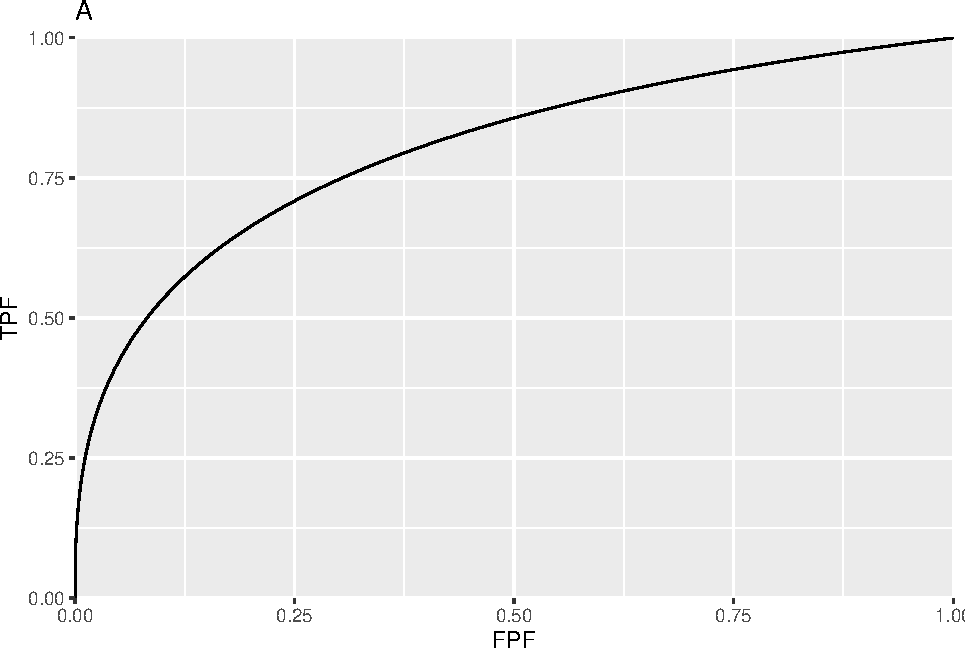
\includegraphics{23-proprocROCs_files/figure-latex/unnamed-chunk-2-1.pdf} 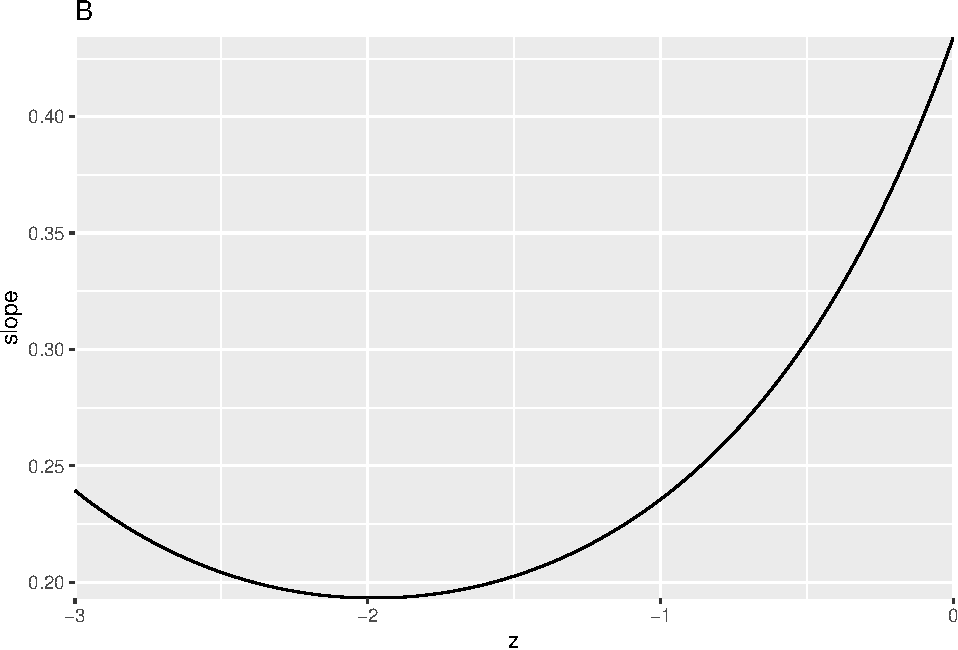
\includegraphics{23-proprocROCs_files/figure-latex/unnamed-chunk-2-2.pdf} 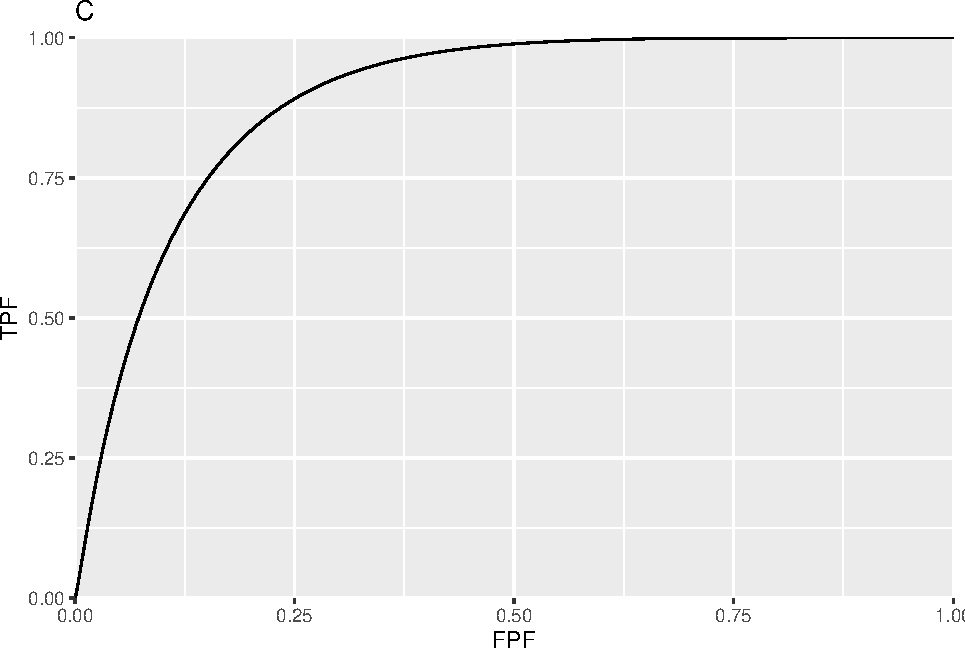
\includegraphics{23-proprocROCs_files/figure-latex/unnamed-chunk-2-3.pdf} 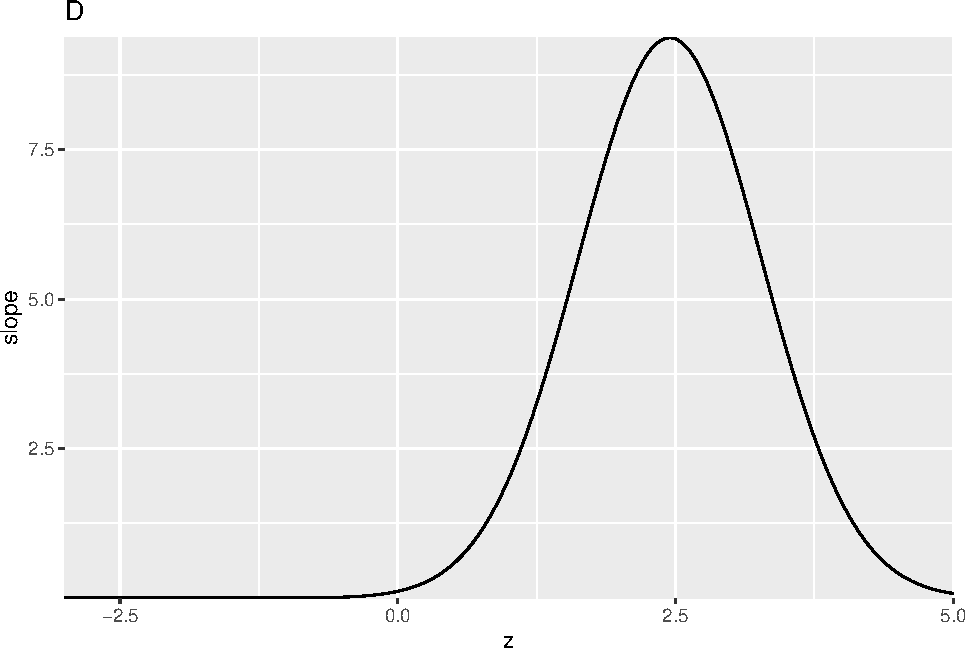
\includegraphics{23-proprocROCs_files/figure-latex/unnamed-chunk-2-4.pdf}

\hypertarget{discussion}{%
\section{Discussion}\label{discussion}}

Plot A is for \texttt{c1} = -0.1322804, \texttt{da} = 1.197239 while plot C is for \texttt{c1} = 0.2225588, \texttt{da} = 1.740157. Plots B and D are the corresponding slope plots as functions of the binormal model z-sample. In plot A, the slope is infinite near the origin and the curve approaches the upper-right corner with finite slope. The situation is reversed in plot C where the slope is finite near the origin and the curve approaches the upper-right corner with zero slope.

These two readers are from a clinical dataset, \texttt{dataset01}. Highest rating inferred ROC data from original FROC data, were analyzed by PROPROC and the resulting parameter values are coded here. They were chosen as they demonstrate key differences in the shapes of proper ROC plots. Plot A corresponds to a negative value of \texttt{c1}, which implies \texttt{b\ \textless{}\ 1}. The slope of the proper ROC is infinite near the origin and approaches a positive constant near the upper right corner of the ROC. Plot C is for a positive value of \texttt{c1}, i.e., for \texttt{b\ \textgreater{}\ 1}. Now the slope of the proper ROC is finite near the origin and approaches zero near the upper right corner.

Considering plot D, as one ``cuts'' the slope axis horizontally with a sliding threshold, starting with very high values and moving downwards, the slope of the ROC curve starts at the origin with a large but finite value. This corresponds to the peak in plot D. Above the peak, there are no solutions for \texttt{z}. The slope decreases monotonically to zero, corresponding to the flattening out of the slope at zero for \texttt{z\ \textasciitilde{}\ \ -2}.

The two values of \texttt{z} corresponding to each cut implies, of course, that the binormal model based proper algorithm has to do a lot of bookkeeping, since each horizontal cut splits the decision axis into 3 regions. One can think of shrinking each of plots B \& D horizontally to zero width, and all that remains is the slope axis with a thick vertical line superimposed on it, corresponding to the horizontally collapsed curves. In plot B the vertical line extends from positive infinity down to about 0.1, and represents the range of decision variable samples encountered by the observer on the likelihood ratio scale. In plot D the vertical line extends from a finite value (\textasciitilde9.4) to zero. For the stated binormal model parameters values outside of these ranges are not possible.

\hypertarget{MetzEqn36}{%
\chapter{Metz Eqn36 numerical check}\label{MetzEqn36}}

\hypertarget{helper-functions-1}{%
\section{Helper functions}\label{helper-functions-1}}

\hypertarget{main-code-and-output-1}{%
\section{Main code and output}\label{main-code-and-output-1}}

\begin{Shaded}
\begin{Highlighting}[]
\NormalTok{npts \textless{}{-}}\StringTok{  }\DecValTok{10000}
\ControlFlowTok{for}\NormalTok{ (i }\ControlFlowTok{in} \DecValTok{1}\OperatorTok{:}\DecValTok{2}\NormalTok{) \{}
  \ControlFlowTok{for}\NormalTok{ (j }\ControlFlowTok{in} \DecValTok{1}\OperatorTok{:}\DecValTok{5}\NormalTok{) \{}
\NormalTok{    C  \textless{}{-}}\StringTok{  }\NormalTok{c1[i,j]}
\NormalTok{    da  \textless{}{-}}\StringTok{  }\NormalTok{d\_a1[i,j]}
\NormalTok{    ret \textless{}{-}}\StringTok{ }\KeywordTok{GetLimits}\NormalTok{(da,C)}
\NormalTok{    LL \textless{}{-}}\StringTok{ }\NormalTok{ret}\OperatorTok{$}\NormalTok{LL;UL \textless{}{-}}\StringTok{ }\NormalTok{ret}\OperatorTok{$}\NormalTok{UL}
\NormalTok{    vc  \textless{}{-}}\StringTok{  }\KeywordTok{seq}\NormalTok{ (LL, UL, }\DataTypeTok{length.out =}\NormalTok{ npts)}
\NormalTok{    TPF  \textless{}{-}}\StringTok{  }\KeywordTok{TruePositiveFraction}\NormalTok{ (vc, da, C)}
\NormalTok{    FPF \textless{}{-}}\StringTok{ }\KeywordTok{FalsePositiveFraction}\NormalTok{ (vc, da, C)}
\NormalTok{    FPF \textless{}{-}}\StringTok{ }\KeywordTok{rev}\NormalTok{(FPF);TPF \textless{}{-}}\StringTok{ }\KeywordTok{rev}\NormalTok{(TPF)}
\NormalTok{    df2 \textless{}{-}}\StringTok{ }\KeywordTok{data.frame}\NormalTok{(}\DataTypeTok{FPF =}\NormalTok{ FPF, }\DataTypeTok{TPF =}\NormalTok{ TPF)}
    \CommentTok{\# do integral numerically}
\NormalTok{    numAuc \textless{}{-}}\StringTok{ }\KeywordTok{trapz}\NormalTok{(FPF, TPF)}
    \CommentTok{\# Implement Eqn. 36 from Metz{-}Pan paper }
\NormalTok{    rho \textless{}{-}}\StringTok{ }\OperatorTok{{-}}\NormalTok{(}\DecValTok{1}\OperatorTok{{-}}\NormalTok{C}\OperatorTok{\^{}}\DecValTok{2}\NormalTok{)}\OperatorTok{/}\NormalTok{(}\DecValTok{1}\OperatorTok{+}\NormalTok{C}\OperatorTok{\^{}}\DecValTok{2}\NormalTok{);sigma \textless{}{-}}\StringTok{ }\KeywordTok{rbind}\NormalTok{(}\KeywordTok{c}\NormalTok{(}\DecValTok{1}\NormalTok{, rho), }\KeywordTok{c}\NormalTok{(rho, }\DecValTok{1}\NormalTok{))}
\NormalTok{    lower \textless{}{-}}\StringTok{ }\KeywordTok{rep}\NormalTok{(}\OperatorTok{{-}}\OtherTok{Inf}\NormalTok{,}\DecValTok{2}\NormalTok{);upper \textless{}{-}}\StringTok{ }\KeywordTok{c}\NormalTok{(}\OperatorTok{{-}}\NormalTok{da}\OperatorTok{/}\KeywordTok{sqrt}\NormalTok{(}\DecValTok{2}\NormalTok{),}\DecValTok{0}\NormalTok{)}
\NormalTok{    aucProproc \textless{}{-}}\StringTok{ }\KeywordTok{pnorm}\NormalTok{(da}\OperatorTok{/}\KeywordTok{sqrt}\NormalTok{(}\DecValTok{2}\NormalTok{)) }\OperatorTok{+}\StringTok{ }\DecValTok{2} \OperatorTok{*}\StringTok{ }\KeywordTok{pmvnorm}\NormalTok{(lower, upper, }\DataTypeTok{sigma =}\NormalTok{ sigma)}
\NormalTok{    aucProproc \textless{}{-}}\StringTok{  }\KeywordTok{as.numeric}\NormalTok{(aucProproc)}
    \KeywordTok{cat}\NormalTok{(}\StringTok{"i = "}\NormalTok{, i,}\StringTok{"j = "}\NormalTok{, j,}\StringTok{"C = "}\NormalTok{, C, }\StringTok{", da = "}\NormalTok{, da, }\StringTok{"aucProproc ="}\NormalTok{, aucProproc, }\StringTok{"Norm. Diff. = "}\NormalTok{, (aucProproc}\OperatorTok{{-}}\NormalTok{numAuc)}\OperatorTok{/}\NormalTok{aucProproc,}\StringTok{"}\CharTok{\textbackslash{}n}\StringTok{"}\NormalTok{)}
\NormalTok{  \}}
\NormalTok{\}}
\CommentTok{\#\textgreater{} i =  1 j =  1 C =  {-}0.1322804 , da =  1.197239 aucProproc = 0.8014164 Norm. Diff. =  3.520017e{-}08 }
\CommentTok{\#\textgreater{} i =  1 j =  2 C =  {-}0.08696513 , da =  1.771176 aucProproc = 0.8947898 Norm. Diff. =  4.741875e{-}08 }
\CommentTok{\#\textgreater{} i =  1 j =  3 C =  {-}0.1444419 , da =  1.481935 aucProproc = 0.8526605 Norm. Diff. =  3.515431e{-}08 }
\CommentTok{\#\textgreater{} i =  1 j =  4 C =  0.08046016 , da =  1.513757 aucProproc = 0.8577776 Norm. Diff. =  4.971428e{-}08 }
\CommentTok{\#\textgreater{} i =  1 j =  5 C =  0.2225588 , da =  1.740157 aucProproc = 0.8909392 Norm. Diff. =  2.699855e{-}08 }
\CommentTok{\#\textgreater{} i =  2 j =  1 C =  {-}0.08174248 , da =  0.6281251 aucProproc = 0.6716574 Norm. Diff. =  2.801793e{-}08 }
\CommentTok{\#\textgreater{} i =  2 j =  2 C =  0.04976448 , da =  0.9738786 aucProproc = 0.7544739 Norm. Diff. =  5.275242e{-}08 }
\CommentTok{\#\textgreater{} i =  2 j =  3 C =  {-}0.1326126 , da =  1.155871 aucProproc = 0.7931787 Norm. Diff. =  3.472577e{-}08 }
\CommentTok{\#\textgreater{} i =  2 j =  4 C =  0.1182226 , da =  1.620176 aucProproc = 0.8740274 Norm. Diff. =  3.922161e{-}08 }
\CommentTok{\#\textgreater{} i =  2 j =  5 C =  0.0781033 , da =  0.8928816 aucProproc = 0.7360989 Norm. Diff. =  3.798459e{-}08}
\end{Highlighting}
\end{Shaded}

\hypertarget{discussion-1}{%
\section{Discussion}\label{discussion-1}}

Note the close correspondence between the formula, Eqn. 36 in the Metz-Pan paper and the numerical estimate. As a historical note, Eqn. 31 and Eqn. 36 (they differ only in parameterizations) in the referenced publication are provided without proof -- it was probably obvious to Prof Metz or he wanted to leave it to us ``mere mortals'' to figure it out, as a final parting gesture of his legacy. The author once put a significant effort into proving it and even had a bright graduate student from the biostatistics department work on it to no avail. The author has observed that these equations always yield very close to the numerical estimates, to within numerical precisions, so the theorem is correct empirically, but he has been unable to prove it analytically. It is left as an exercise for a gifted reader to prove/disprove these equations.

\hypertarget{CbmPlots}{%
\chapter{CBM Plots}\label{CbmPlots}}

\hypertarget{helper-functions-2}{%
\section{Helper functions}\label{helper-functions-2}}

\hypertarget{main-code-and-output-2}{%
\section{Main code and output}\label{main-code-and-output-2}}

\begin{verbatim}
#> Fig. A : mu =  1 , alpha =  0.2
#> Fig. B : mu =  3 , alpha =  0.2
#> Fig. C : mu =  1 , alpha =  0.8
#> Fig. D : mu =  3 , alpha =  0.8
\end{verbatim}

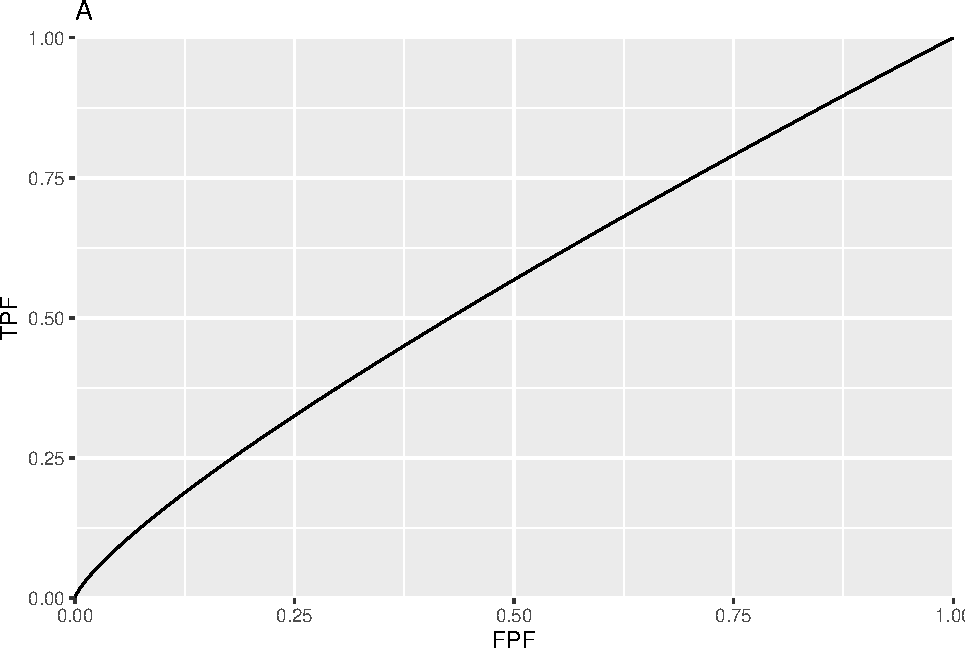
\includegraphics{31-cbmPlots_files/figure-latex/unnamed-chunk-2-1.pdf} 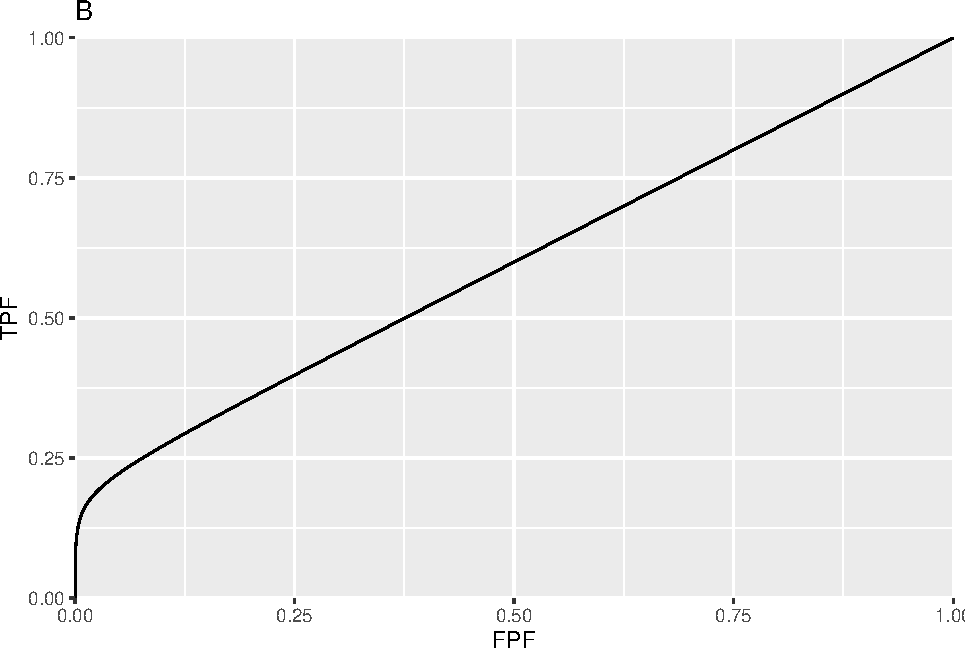
\includegraphics{31-cbmPlots_files/figure-latex/unnamed-chunk-2-2.pdf} 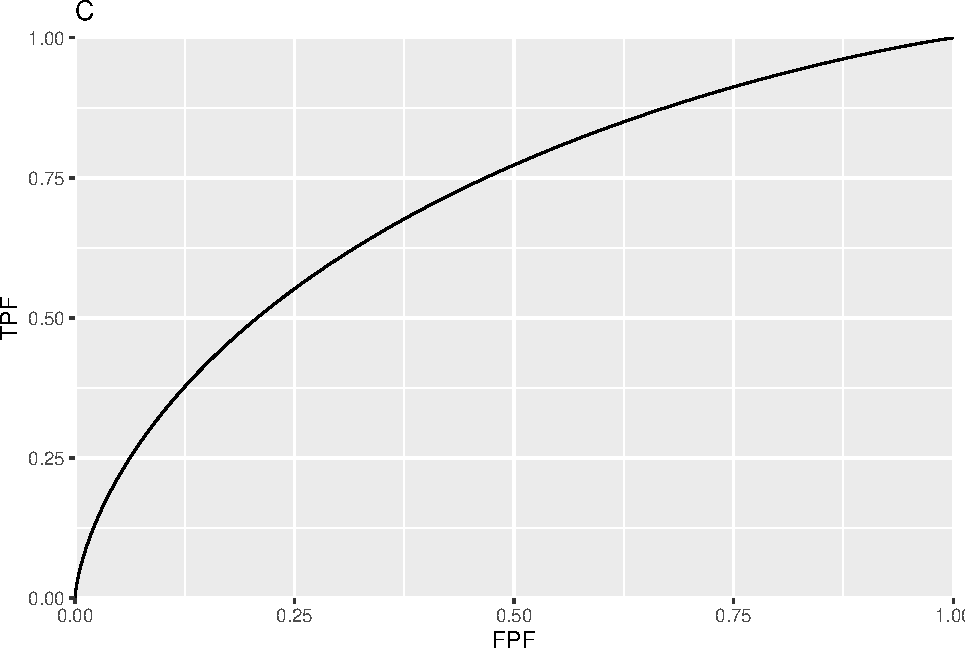
\includegraphics{31-cbmPlots_files/figure-latex/unnamed-chunk-2-3.pdf} 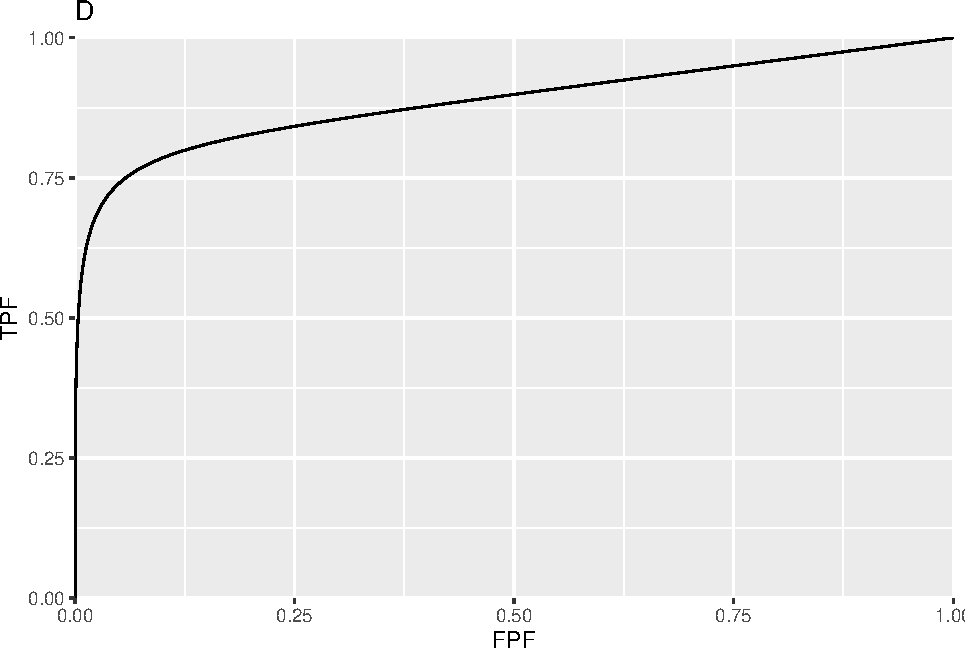
\includegraphics{31-cbmPlots_files/figure-latex/unnamed-chunk-2-4.pdf}

\hypertarget{comments-3}{%
\section{Comments}\label{comments-3}}

Plots A - D show ROC curves predicted by the CBM model; the corresponding values of the \(mu\) and \(alpha\) parameters are indicated above the plots. For small \(mu\) and/or \(alpha\) the curve approaches the chance diagonal, consistent with the notion that if the lesion is not visible, performance can be no better than chance level.

\hypertarget{pdf-plots}{%
\section{pdf plots}\label{pdf-plots}}

\begin{verbatim}
#> Fig. E : mu =  1 , alpha =  0.2
#> Fig. F : mu =  3 , alpha =  0.2
#> Fig. G : mu =  1 , alpha =  0.8
#> Fig. H : mu =  3 , alpha =  0.8
\end{verbatim}

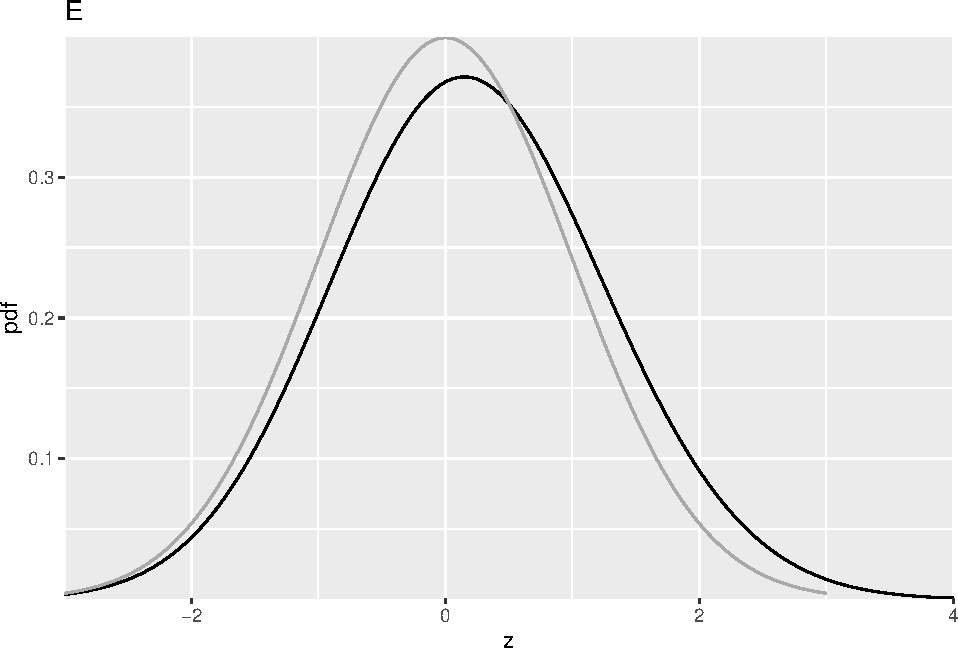
\includegraphics{31-cbmPlots_files/figure-latex/unnamed-chunk-3-1.pdf} 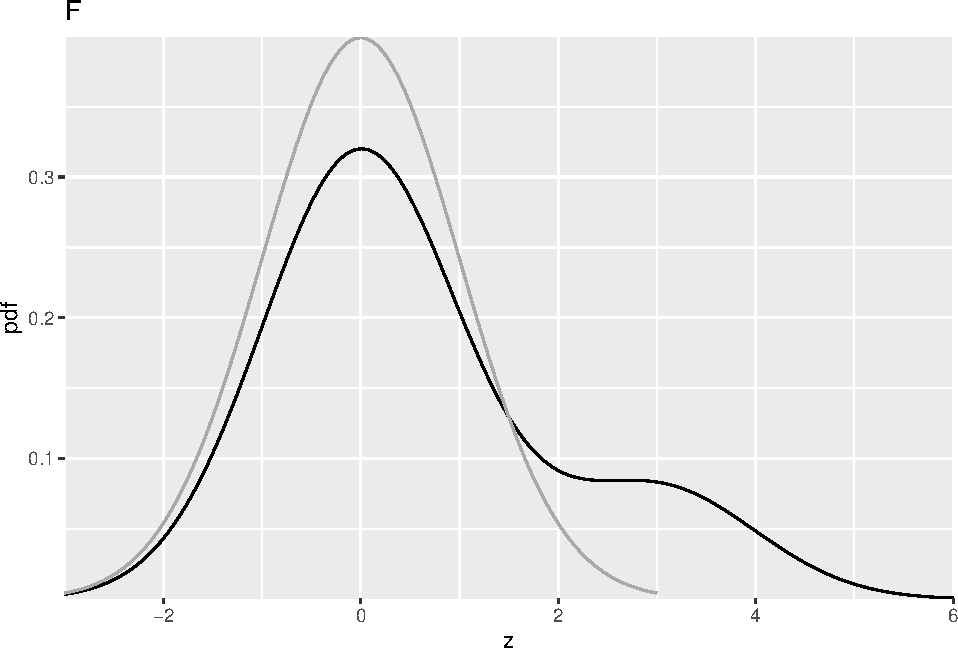
\includegraphics{31-cbmPlots_files/figure-latex/unnamed-chunk-3-2.pdf} 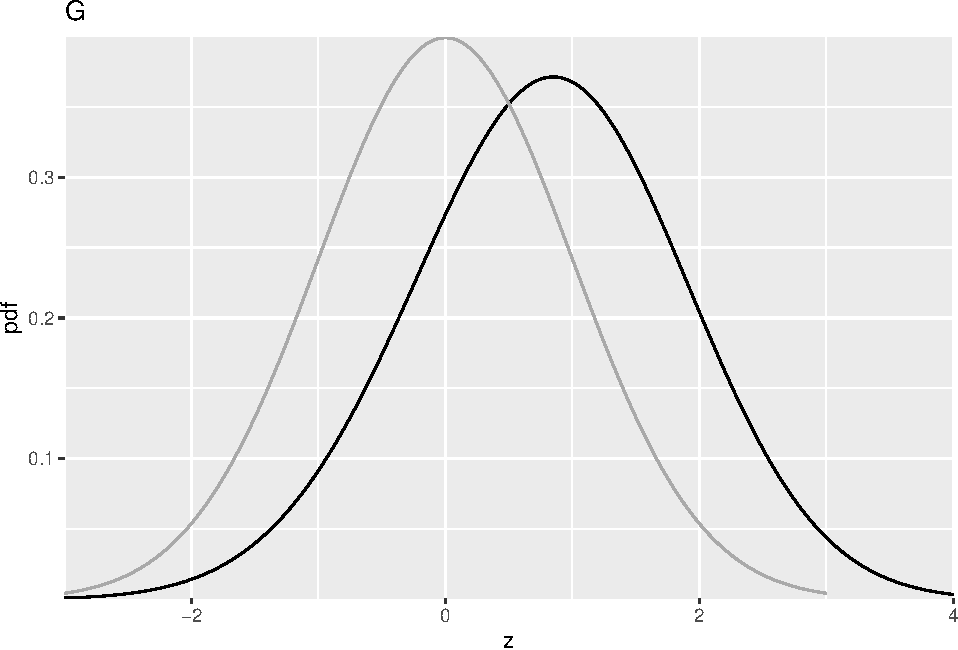
\includegraphics{31-cbmPlots_files/figure-latex/unnamed-chunk-3-3.pdf} 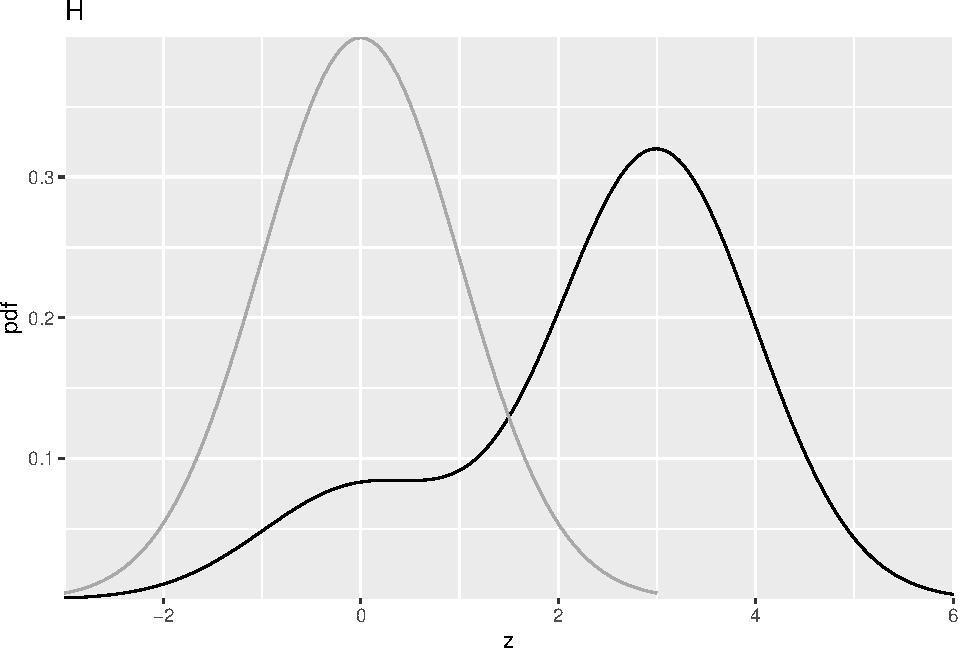
\includegraphics{31-cbmPlots_files/figure-latex/unnamed-chunk-3-4.pdf}

\hypertarget{comments-4}{%
\section{Comments}\label{comments-4}}

The dark line is the diseased distribution. The grey line is the non-diseased distribution. The bimodal diseased distribution is clearly evident in plots F and H.

\hypertarget{likelihood-ratio-plots}{%
\section{likelihood ratio plots}\label{likelihood-ratio-plots}}

\begin{verbatim}
#> Fig. I : mu =  1 , alpha =  0.2
#> Fig. J : mu =  3 , alpha =  0.2
#> Fig. K : mu =  1 , alpha =  0.8
#> Fig. L : mu =  3 , alpha =  0.8
\end{verbatim}

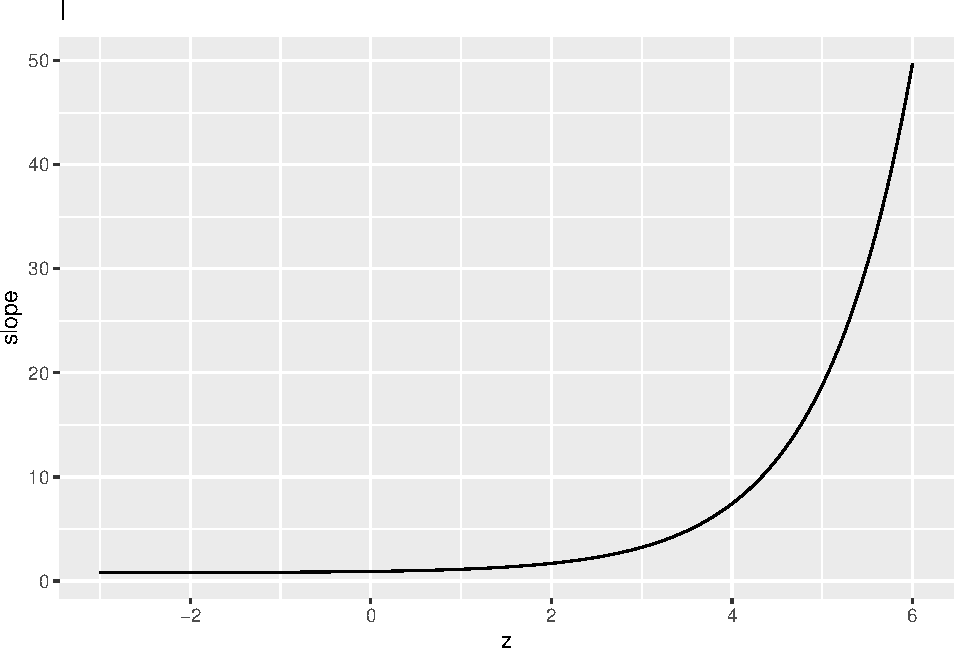
\includegraphics{31-cbmPlots_files/figure-latex/unnamed-chunk-4-1.pdf} 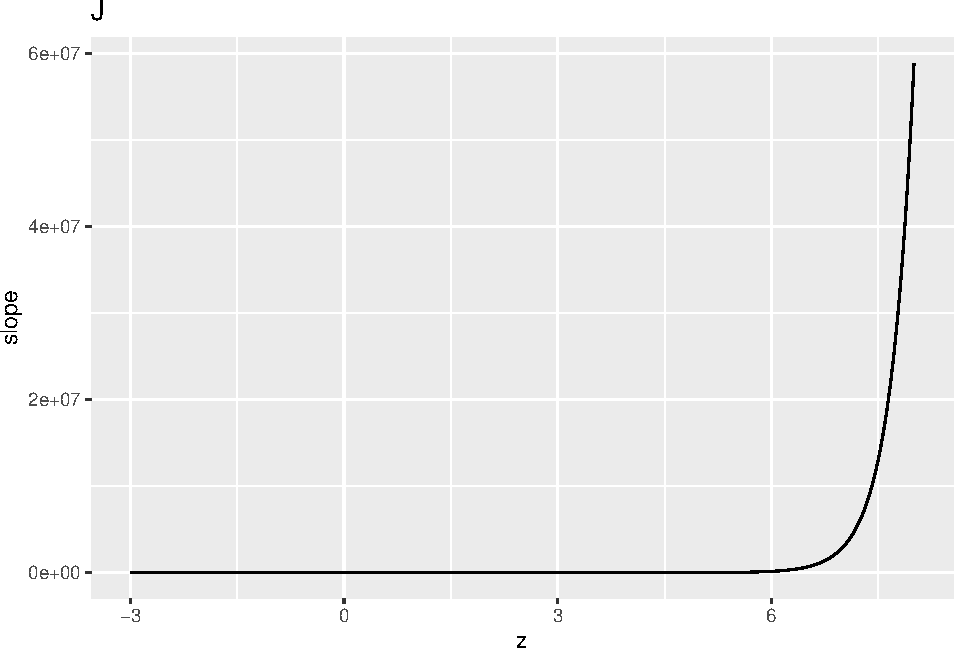
\includegraphics{31-cbmPlots_files/figure-latex/unnamed-chunk-4-2.pdf} 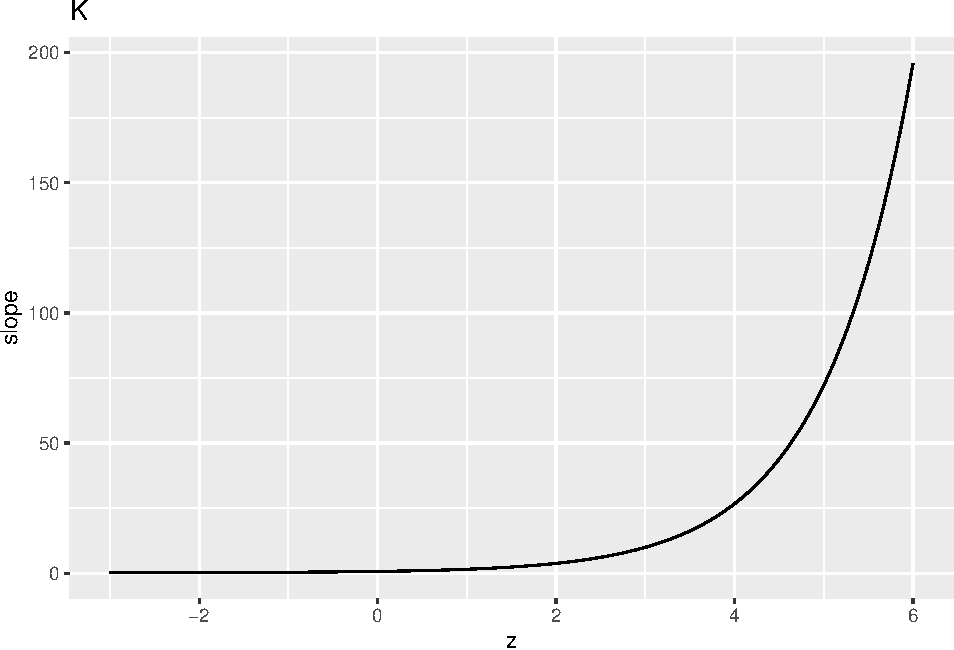
\includegraphics{31-cbmPlots_files/figure-latex/unnamed-chunk-4-3.pdf} 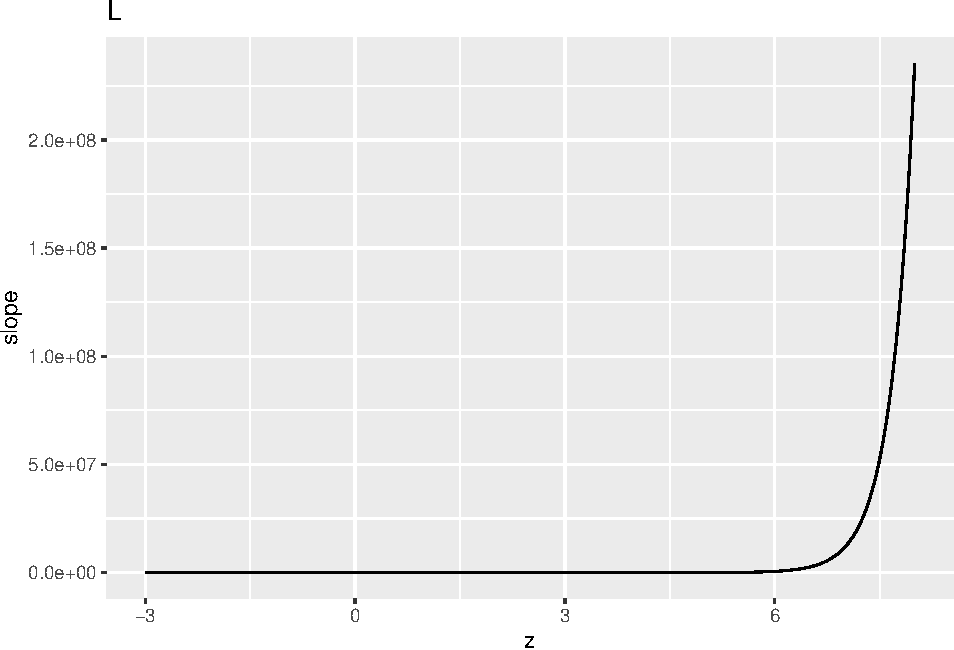
\includegraphics{31-cbmPlots_files/figure-latex/unnamed-chunk-4-4.pdf}

\hypertarget{comments-5}{%
\section{Comments}\label{comments-5}}

Close examination of the region near the flat part shows it does not plateau at zero; rather the minimum is at 1 - \(alpha\), explaining the non-zero limiting slope of the predicted curve near (1, 1).

\hypertarget{ROIDataStr}{%
\chapter{ROI paradigm data}\label{ROIDataStr}}

\hypertarget{introduction-this-vignette-is-under-construction}{%
\section{Introduction; this vignette is under construction!}\label{introduction-this-vignette-is-under-construction}}

\begin{itemize}
\tightlist
\item
  In the region-of-interest (ROI) paradigm \citep[\citet{RN55}]{RN1233} each case is regarded as consisting of \({Q_{k}}\) (\({Q_{k}}\ge 1\)) ``quadrants'' or ``regions-of-interest'' or ROIs, where \emph{k} is the case index (\(k=1,2,...,K\)) and \(K\) is the total number of cases (i.e., case-level non-diseased plus case-level diseased cases). Each ROI needs to be classified, by the investigator, as either ROI-level-non-diseased (i.e., it has no lesions) or ROI-level-diseased (i.e., it has at least one lesion). \textbf{Note the distinction between case-level and ROI-level truth states.} One can have ROI-level non-diseased regions in a case-level diseased case. A case-level diseased case must contain at least one ROI-level diseased region and a case-level non-diseased case cannot have any ROI-level diseased regions.
\item
  The observer gives a single rating (in fact an ordered label) to each ROI, denoted \({R_{kr}}\) (\(r\) = 1, 2, \ldots, \({Q_k}\)). Here \(r\) is the ROI index and \(k\) is the case index. The rating can be an integer or quasi- continuous (e.g., 0 -- 100), or a floating point value, as long as higher numbers represent greater confidence in presence of one or more lesions in the ROI.
\item
  The ROI paradigm is not restricted to 4 or even a constant number of ROIs per case. That is the reason for the \emph{k} subscript in \({Q_k}\).
\item
  The ROI data structure is a special case of the FROC data structure, the essential difference being that the number of ratings per case is an a-priori known value, equal to \({Q_{k}}\).
\item
  ROI-level non-diseased region ratings are stored in the \texttt{NL} field and ROI-level diseased region ratings are stored in the \texttt{LL} field.\\
\item
  One can think of the ROI paradigm as similar to the FROC paradigm, but with localization accuracy restricted to belonging to a region (one cannot distinguish multiple lesions within a region). Unlike the FROC paradigm, a rating \emph{is required} for every ROI.
\end{itemize}

\hypertarget{an-example-roi-dataset}{%
\section{An example ROI dataset}\label{an-example-roi-dataset}}

An example simulated ROI dataset is included as \texttt{datasetROI}.

\begin{Shaded}
\begin{Highlighting}[]
\KeywordTok{str}\NormalTok{(datasetROI)}
\CommentTok{\#\textgreater{} List of 8}
\CommentTok{\#\textgreater{}  $ NL          : num [1:2, 1:5, 1:90, 1:4] 0.95 0.927 0.556 0.805 1.421 ...}
\CommentTok{\#\textgreater{}  $ LL          : num [1:2, 1:5, 1:40, 1:4] 1.57 2.31 2.3 2.34 2.34 ...}
\CommentTok{\#\textgreater{}  $ lesionVector: int [1:40] 2 3 2 2 3 3 1 2 3 3 ...}
\CommentTok{\#\textgreater{}  $ lesionID    : num [1:40, 1:4] 2 1 1 1 1 2 4 1 1 1 ...}
\CommentTok{\#\textgreater{}  $ lesionWeight: num [1:40, 1:4] 0.5 0.333 0.5 0.5 0.333 ...}
\CommentTok{\#\textgreater{}  $ dataType    : chr "ROI"}
\CommentTok{\#\textgreater{}  $ modalityID  : Named chr [1:2] "1" "2"}
\CommentTok{\#\textgreater{}   ..{-} attr(*, "names")= chr [1:2] "1" "2"}
\CommentTok{\#\textgreater{}  $ readerID    : Named chr [1:5] "1" "2" "3" "4" ...}
\CommentTok{\#\textgreater{}   ..{-} attr(*, "names")= chr [1:5] "1" "2" "3" "4" ...}
\NormalTok{datasetROI}\OperatorTok{$}\NormalTok{NL[}\DecValTok{1}\NormalTok{,}\DecValTok{1}\NormalTok{,}\DecValTok{1}\NormalTok{,]}
\CommentTok{\#\textgreater{} [1]  0.9498680 {-}0.0582497 {-}0.7763780  0.0120730}
\KeywordTok{mean}\NormalTok{(datasetROI}\OperatorTok{$}\NormalTok{NL[,,}\DecValTok{1}\OperatorTok{:}\DecValTok{50}\NormalTok{,])}
\CommentTok{\#\textgreater{} [1] 0.1014348}
\NormalTok{datasetROI}\OperatorTok{$}\NormalTok{NL[}\DecValTok{1}\NormalTok{,}\DecValTok{1}\NormalTok{,}\DecValTok{51}\NormalTok{,]}
\CommentTok{\#\textgreater{} [1] 1.01867 0.34710    {-}Inf    {-}Inf}
\NormalTok{datasetROI}\OperatorTok{$}\NormalTok{lesionVector[}\DecValTok{1}\NormalTok{]}
\CommentTok{\#\textgreater{} [1] 2}
\NormalTok{datasetROI}\OperatorTok{$}\NormalTok{LL[}\DecValTok{1}\NormalTok{,}\DecValTok{1}\NormalTok{,}\DecValTok{1}\NormalTok{,]}
\CommentTok{\#\textgreater{} [1] 1.56928 2.05945    {-}Inf    {-}Inf}
\NormalTok{x \textless{}{-}}\StringTok{ }\NormalTok{datasetROI}\OperatorTok{$}\NormalTok{LL;}\KeywordTok{mean}\NormalTok{(x[}\KeywordTok{is.finite}\NormalTok{(x)])}
\CommentTok{\#\textgreater{} [1] 1.815513}
\end{Highlighting}
\end{Shaded}

Examination of the output reveals that:

\begin{itemize}
\tightlist
\item
  This is a 2-treatment 5-reader dataset, with 50 non-diseased cases and 40 diseased cases, and \({Q_k}=4\) for all \emph{k}.\\
\item
  For treatment 1, reader 1, case 1 (the 1st non-diseased case) the 4 ratings are 0.949868, -0.0582497, -0.776378, 0.012073. The mean of all ratings on non-diseased cases is 0.1014348.\\
\item
  For treatment 1, reader 1, case 51 (the 1st diseased case) the NL ratings are 1.01867, 0.3471. There are only two finite values because this case has two ROI-level-diseased regions, and 2 plus 2 makes for the assumed 4-regions per case. The corresponding \texttt{\$lesionVector} field is 2.\\
\item
  The ratings of the 2 ROI-level-diseased ROIs on this case are 1.56928, 2.05945. The mean rating over all ROI-level-diseased ROIs is 1.8155127.
\end{itemize}

\hypertarget{the-roi-excel-data-file}{%
\section{The ROI Excel data file}\label{the-roi-excel-data-file}}

\begin{itemize}
\tightlist
\item
  An Excel file in JAFROC format containing simulated ROI data corresponding to \texttt{datasetROI}, is included with the distribution. The first command (below) finds the location of the file and the second command reads it and saves it to a dataset object \texttt{ds}. !!!DPC!!!
\item
  The \texttt{DfReadDataFile} function automatically recognizes that this is an \emph{ROI} dataset. Its structure is similar to the JAFROC format Excel file, with some important differences, noted below. It contains three worksheets:
\end{itemize}

\begin{Shaded}
\begin{Highlighting}[]
\CommentTok{\#\# fileName \textless{}{-} system.file(}
\CommentTok{\#\#     "extdata", "RoiData.xlsx", package = "RJafroc", mustWork = TRUE)}
\CommentTok{\#\# ds \textless{}{-} DfReadDataFile(fileName)}
\CommentTok{\#\# ds$dataType}
\end{Highlighting}
\end{Shaded}

\begin{figure}

{\centering 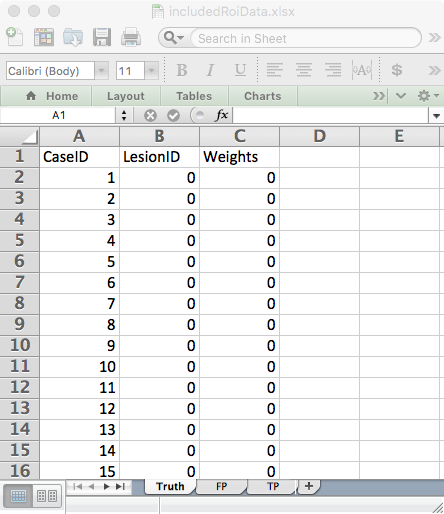
\includegraphics[width=0.5\linewidth,height=0.2\textheight]{images/ROI-Truth-1} 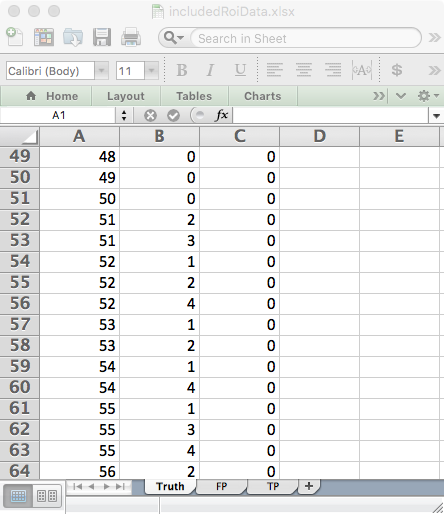
\includegraphics[width=0.5\linewidth,height=0.2\textheight]{images/ROI-Truth-2} 

}

\caption{Fig. 1 two views of Truth worksheet}\label{fig:unnamed-chunk-3}
\end{figure}

\begin{itemize}
\tightlist
\item
  The \texttt{Truth} worksheet, Fig. 1, indicates which cases are diseased and which are non-diseased and the number of ROI-level-diseased region on each case.

  \begin{itemize}
  \tightlist
  \item
    There are 50 non-diseased cases (labeled 1-50) under column \texttt{CaseID} and 40 diseased cases (labeled 51-90).\\
  \item
    The \texttt{LesionID} field for each non-diseased case (e.g., \texttt{CaseID} = 1) is zero and there is one row per case. For diseased cases, this field has a variable number of entries, ranging from 1 to 4. As an example, there are two rows for \texttt{CaseID} = 51 in the Excel file: one with \texttt{LesionID} = 2 and one with \texttt{LesionID} = 3.\\
  \item
    The \texttt{Weights} field is always zero (this field is not used in ROI analysis).
  \end{itemize}
\end{itemize}

\begin{figure}

{\centering 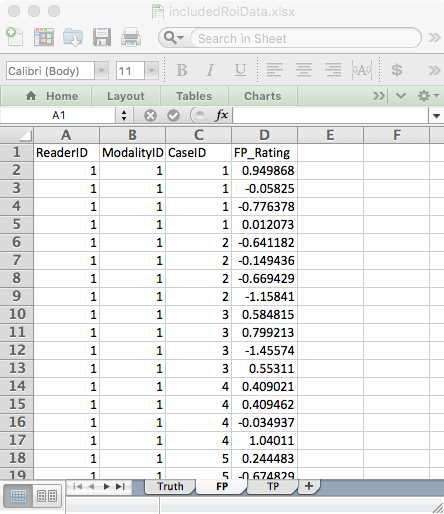
\includegraphics[width=0.5\linewidth,height=0.2\textheight]{images/ROI-FP-1} 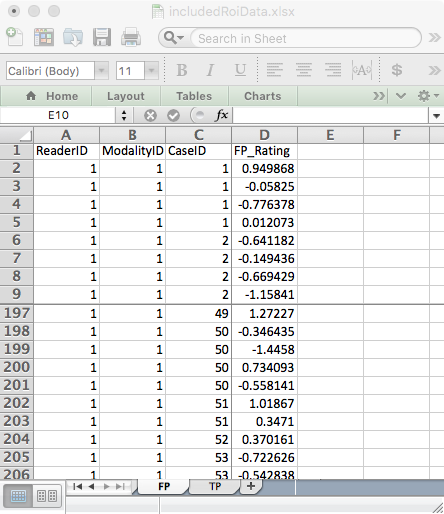
\includegraphics[width=0.5\linewidth,height=0.2\textheight]{images/ROI-FP-2} 

}

\caption{Fig. 2 two views of FP worksheet}\label{fig:unnamed-chunk-4}
\end{figure}

\begin{itemize}
\tightlist
\item
  The \texttt{FP} (or \texttt{NL}) worksheet - this lists the ratings of ROI-level-non-diseased regions.

  \begin{itemize}
  \tightlist
  \item
    For \texttt{ReaderID} = 1, \texttt{ModalityID} = 1 and \texttt{CaseID} = 1 there are 4 rows, corresponding to the 4 ROI-level-non-diseased regions in this case. The corresponding ratings are 0.949868, -0.0582497, -0.776378, 0.012073. The pattern repeats for other treatments and readers, but the rating are, of course, different.\\
  \item
    Each \texttt{CaseID} is represented in the \texttt{FP} worksheet (a rare exception could occur if a case-level diseased case has 4 diseased regions).
  \end{itemize}
\end{itemize}

\begin{figure}

{\centering 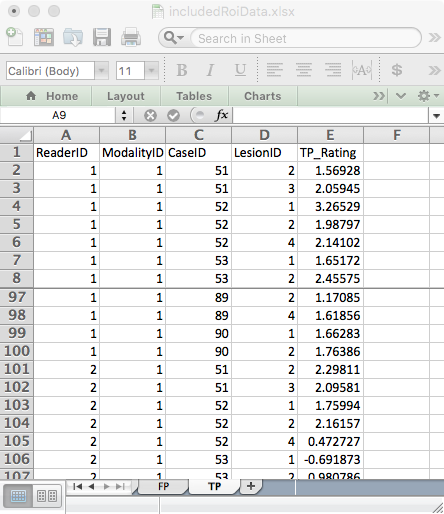
\includegraphics[width=0.5\linewidth,height=0.2\textheight]{images/ROI-TP-1} 

}

\caption{Fig. 2 TP worksheet}\label{fig:unnamed-chunk-5}
\end{figure}

\begin{itemize}
\tightlist
\item
  The \texttt{TP} (or \texttt{LL}) worksheet - this lists the ratings of ROI-level-diseased regions.

  \begin{itemize}
  \tightlist
  \item
    Because non-diseased cases generate TPs, one does not find any entry with \texttt{CaseID} = 1-50 in the \texttt{TP} worksheet.\\
  \item
    The lowest \texttt{CaseID} in the \texttt{TP} worksheet is 51, which corresponds to the first diseased case.\\
  \item
    There are two entries for this case, corresponding to the two ROI-level-diseased regions present in this case. Recall that corresponding to this \texttt{CaseID} in the \texttt{Truth} worksheet there were two entries with \texttt{LesionID} = 2 and 3. These must match the \texttt{LesionID}'s listed for this case in the \texttt{TP} worksheet. Complementing these two entries, in the \texttt{FP} worksheet for \texttt{CaseID} = 51, there are 2 entries corresponding to the two ROI-level-non-diseased regions in this case.\\
  \item
    One should confirm that for each diseased case the sum of the number of entries in the \texttt{TP} and \texttt{FP} worksheets is always 4.
  \end{itemize}
\end{itemize}

\hypertarget{next-tba}{%
\section{Next, TBA}\label{next-tba}}

The next vignette illustrates significance testing for this paradigm.

\hypertarget{references-4}{%
\section{References}\label{references-4}}

\hypertarget{ROIDataAnalysis}{%
\chapter{Analyzing data acquired according to the ROI paradigm}\label{ROIDataAnalysis}}

\hypertarget{introduction-this-vignette-is-under-construction-1}{%
\section{Introduction; this vignette is under construction!}\label{introduction-this-vignette-is-under-construction-1}}

\hypertarget{note-to-self-102919-dpc}{%
\section{Note to self (10/29/19) !!!DPC!!!}\label{note-to-self-102919-dpc}}

The FOM and DeLong method implementations need checking with a toy dataset.

\hypertarget{introduction-3}{%
\section{Introduction}\label{introduction-3}}

\begin{itemize}
\item
  For an ROI dataset \texttt{StSignificanceTesting()} automatically defaults to \texttt{method\ =\ "ORH"}, \texttt{covEstMethod\ =\ "DeLong"} and \texttt{FOM\ =\ "ROI"}.
\item
  The covariance estimation method is based on the original DeLong method \citep{RN112}, which is valid only for the trapezoidal AUC, i.e.~ROC data, as extended by \citep{RN1233} to ROI data, see formula below.
\item
  The essential differences from conventional ROC analyses are in the definition of the ROI figure of merit, see below, and the procedure developed by \citep{RN1233} for estimating the covariance matrix. Once the covariances are known, \texttt{method\ =\ "ORH"} can be applied to perform significance testing, as described in \citep{RN1450} and \citep[Chapter 10]{RN2680}.
\end{itemize}

\hypertarget{the-roi-figure-of-merit}{%
\section{The ROI figure of merit}\label{the-roi-figure-of-merit}}

Let \({X_{kr}}\) denote the rating for the r\textsuperscript{th} \textbf{lesion-containing} ROI in the k\textsuperscript{th} case and let \(n_{k}^L\) be the total number of lesion-containing ROIs in the k\textsuperscript{th} case. Similarly, let \({Y_{kr}}\) denote the rating for the r\textsuperscript{th} \textbf{lesion-free} ROI in the k\textsuperscript{th} case and \(n_{k}^N\) denote the total number of lesion-free ROIs in the k\textsuperscript{th} case. Let \({N_L}\) denote the total number of lesion-containing ROIs in the image set and \(N_N\) denote the total number of lesion-free ROIs. These are given by:
\[N_L=\sum\nolimits_{k}{n_{k}^L}\] and \[N_N=\sum\nolimits_{k}{n_{k}^N}\]
The ROI figure of merit \(\theta\) is defined by:

\begin{equation*} 
\theta =\frac{1}{N_LN_N}\sum\nolimits_k{\sum\nolimits_{k'}{\sum\limits_{r=1}^{n_{k}^{L}}{\sum\limits_{r'=1}^{n_{k'}^{N}}{\psi (X_{kr},{Y_{k'r'}})}}}}
\end{equation*}

The kernel function \(\Psi(X,Y)\) is defined by:

\begin{equation*} 
\psi\left ( X,Y \right ) =\begin{bmatrix}
1 &    \text{if}& {X < Y}\\ 
0.5 &  \text{if}& {X = Y}\\ 
 0 &   \text{if}& {X > Y} 
\end{bmatrix}
\end{equation*}

The ROIs are \emph{effectively regarded as mini-cases} and one calculates the FOM as the Wilcoxon statistic considering the mini-cases as actual cases. The correlations between the ratings of ROIs on the same case are accounted for in the analysis.

\hypertarget{calculation-of-the-roi-figure-of-merit.}{%
\section{Calculation of the ROI figure of merit.}\label{calculation-of-the-roi-figure-of-merit.}}

\begin{Shaded}
\begin{Highlighting}[]
\KeywordTok{UtilFigureOfMerit}\NormalTok{(datasetROI, }\DataTypeTok{FOM =} \StringTok{"ROI"}\NormalTok{)}
\CommentTok{\#\textgreater{}           Rdr1      Rdr2      Rdr3      Rdr4      Rdr5}
\CommentTok{\#\textgreater{} Trt1 0.9057239 0.8842834 0.8579279 0.9350207 0.8352103}
\CommentTok{\#\textgreater{} Trt2 0.9297186 0.9546035 0.8937652 0.9531716 0.8770076}
\NormalTok{fom \textless{}{-}}\StringTok{ }\KeywordTok{UtilFigureOfMerit}\NormalTok{(datasetROI, }\DataTypeTok{FOM =} \StringTok{"ROI"}\NormalTok{)}
\end{Highlighting}
\end{Shaded}

\begin{itemize}
\tightlist
\item
  If the correct \texttt{FOM} is not supplied, it defaults to \texttt{FOM\ =\ ROI}.\\
\item
  This is a 2-treatment 5-reader dataset.\\
\item
  For treatment 1, reader 1 the figure of merit is 0.9057239.\\
\item
  For treatment 2, reader 5 the figure of merit is 0.8770076.\\
\item
  Etc.
\end{itemize}

\hypertarget{significance-testing}{%
\section{Significance testing}\label{significance-testing}}

When \texttt{dataset\$dataType\ ==\ "ROI"} the FOM defaults to ``ROI'' (meaning the above formula) and the covariance estimation method defaults to \texttt{covEstMethod\ =\ "DeLong"}.

\begin{Shaded}
\begin{Highlighting}[]
\NormalTok{ret \textless{}{-}}\StringTok{ }\KeywordTok{StSignificanceTesting}\NormalTok{(datasetROI, }\DataTypeTok{FOM =} \StringTok{"Wilcoxon"}\NormalTok{)}
\CommentTok{\#\textgreater{} ROI dataset: forcing method = \textasciigrave{}ORH\textasciigrave{}, covEstMethod = \textasciigrave{}DeLong\textasciigrave{} and FOM = \textasciigrave{}ROI\textasciigrave{}.}
\KeywordTok{str}\NormalTok{(ret)}
\CommentTok{\#\textgreater{} List of 14}
\CommentTok{\#\textgreater{}  $ fomArray            : num [1:2, 1:5] 0.906 0.93 0.884 0.955 0.858 ...}
\CommentTok{\#\textgreater{}   ..{-} attr(*, "dimnames")=List of 2}
\CommentTok{\#\textgreater{}   .. ..$ : chr [1:2] "Trt1" "Trt2"}
\CommentTok{\#\textgreater{}   .. ..$ : chr [1:5] "Rdr1" "Rdr2" "Rdr3" "Rdr4" ...}
\CommentTok{\#\textgreater{}  $ meanSquares         :\textquotesingle{}data.frame\textquotesingle{}:    1 obs. of  3 variables:}
\CommentTok{\#\textgreater{}   ..$ msT : num 0.00361}
\CommentTok{\#\textgreater{}   ..$ msR : num 0.00256}
\CommentTok{\#\textgreater{}   ..$ msTR: num 0.000207}
\CommentTok{\#\textgreater{}  $ varComp             :\textquotesingle{}data.frame\textquotesingle{}:    1 obs. of  6 variables:}
\CommentTok{\#\textgreater{}   ..$ varR : num 0.00108}
\CommentTok{\#\textgreater{}   ..$ varTR: num 0.000153}
\CommentTok{\#\textgreater{}   ..$ cov1 : num 0.000247}
\CommentTok{\#\textgreater{}   ..$ cov2 : num 0.000187}
\CommentTok{\#\textgreater{}   ..$ cov3 : num 0.000154}
\CommentTok{\#\textgreater{}   ..$ var  : num 0.000333}
\CommentTok{\#\textgreater{}  $ FTestStatsRRRC      :\textquotesingle{}data.frame\textquotesingle{}:    1 obs. of  4 variables:}
\CommentTok{\#\textgreater{}   ..$ fRRRC  : num 9.76}
\CommentTok{\#\textgreater{}   ..$ ndfRRRC: num 1}
\CommentTok{\#\textgreater{}   ..$ ddfRRRC: num 12.8}
\CommentTok{\#\textgreater{}   ..$ pRRRC  : num 0.00817}
\CommentTok{\#\textgreater{}  $ ciDiffTrtRRRC       :\textquotesingle{}data.frame\textquotesingle{}:    1 obs. of  8 variables:}
\CommentTok{\#\textgreater{}   ..$ Treatment: chr "Trt1{-}Trt2"}
\CommentTok{\#\textgreater{}   ..$ Estimate : num {-}0.038}
\CommentTok{\#\textgreater{}   ..$ StdErr   : num 0.0122}
\CommentTok{\#\textgreater{}   ..$ DF       : num 12.8}
\CommentTok{\#\textgreater{}   ..$ t        : num {-}3.12}
\CommentTok{\#\textgreater{}   ..$ PrGTt    : num 0.00817}
\CommentTok{\#\textgreater{}   ..$ CILower  : num {-}0.0643}
\CommentTok{\#\textgreater{}   ..$ CIUpper  : num {-}0.0117}
\CommentTok{\#\textgreater{}  $ ciAvgRdrEachTrtRRRC :\textquotesingle{}data.frame\textquotesingle{}:    2 obs. of  6 variables:}
\CommentTok{\#\textgreater{}   ..$ Treatment: Factor w/ 2 levels "Trt1","Trt2": 1 2}
\CommentTok{\#\textgreater{}   ..$ Area     : num [1:2] 0.884 0.922}
\CommentTok{\#\textgreater{}   ..$ StdErr   : num [1:2] 0.0232 0.0197}
\CommentTok{\#\textgreater{}   ..$ DF       : num [1:2] 12.2 10.1}
\CommentTok{\#\textgreater{}   ..$ CILower  : num [1:2] 0.833 0.878}
\CommentTok{\#\textgreater{}   ..$ CIUpper  : num [1:2] 0.934 0.966}
\CommentTok{\#\textgreater{}  $ FTestStatsFRRC      :\textquotesingle{}data.frame\textquotesingle{}:    1 obs. of  4 variables:}
\CommentTok{\#\textgreater{}   ..$ fFRRC  : num 16.6}
\CommentTok{\#\textgreater{}   ..$ ndfFRRC: num 1}
\CommentTok{\#\textgreater{}   ..$ ddfFRRC: num Inf}
\CommentTok{\#\textgreater{}   ..$ pFRRC  : num 4.58e{-}05}
\CommentTok{\#\textgreater{}  $ ciDiffTrtFRRC       :\textquotesingle{}data.frame\textquotesingle{}:    1 obs. of  8 variables:}
\CommentTok{\#\textgreater{}   ..$ Treatment: chr "Trt1{-}Trt2"}
\CommentTok{\#\textgreater{}   ..$ Estimate : num {-}0.038}
\CommentTok{\#\textgreater{}   ..$ StdErr   : num 0.00933}
\CommentTok{\#\textgreater{}   ..$ DF       : num Inf}
\CommentTok{\#\textgreater{}   ..$ t        : num {-}4.08}
\CommentTok{\#\textgreater{}   ..$ PrGTt    : num 4.58e{-}05}
\CommentTok{\#\textgreater{}   ..$ CILower  : num {-}0.0563}
\CommentTok{\#\textgreater{}   ..$ CIUpper  : num {-}0.0197}
\CommentTok{\#\textgreater{}  $ ciAvgRdrEachTrtFRRC :\textquotesingle{}data.frame\textquotesingle{}:    2 obs. of  6 variables:}
\CommentTok{\#\textgreater{}   ..$ Treatment: Factor w/ 2 levels "Trt1","Trt2": 1 2}
\CommentTok{\#\textgreater{}   ..$ Area     : num [1:2] 0.884 0.922}
\CommentTok{\#\textgreater{}   ..$ StdErr   : num [1:2] 0.0163 0.0129}
\CommentTok{\#\textgreater{}   ..$ DF       : num [1:2] Inf Inf}
\CommentTok{\#\textgreater{}   ..$ CILower  : num [1:2] 0.852 0.896}
\CommentTok{\#\textgreater{}   ..$ CIUpper  : num [1:2] 0.916 0.947}
\CommentTok{\#\textgreater{}  $ ciDiffTrtEachRdrFRRC:\textquotesingle{}data.frame\textquotesingle{}:    5 obs. of  9 variables:}
\CommentTok{\#\textgreater{}   ..$ Reader   : Factor w/ 5 levels "Rdr1","Rdr2",..: 1 2 3 4 5}
\CommentTok{\#\textgreater{}   ..$ Treatment: Factor w/ 1 level "Trt1{-}Trt2": 1 1 1 1 1}
\CommentTok{\#\textgreater{}   ..$ Estimate : num [1:5] {-}0.024 {-}0.0703 {-}0.0358 {-}0.0182 {-}0.0418}
\CommentTok{\#\textgreater{}   ..$ StdErr   : num [1:5] 0.01025 0.01448 0.01648 0.00928 0.01398}
\CommentTok{\#\textgreater{}   ..$ DF       : num [1:5] Inf Inf Inf Inf Inf}
\CommentTok{\#\textgreater{}   ..$ t        : num [1:5] {-}2.34 {-}4.86 {-}2.17 {-}1.96 {-}2.99}
\CommentTok{\#\textgreater{}   ..$ PrGTt    : num [1:5] 1.93e{-}02 1.20e{-}06 2.97e{-}02 5.05e{-}02 2.79e{-}03}
\CommentTok{\#\textgreater{}   ..$ CILower  : num [1:5] {-}0.0441 {-}0.0987 {-}0.0681 {-}0.0363 {-}0.0692}
\CommentTok{\#\textgreater{}   ..$ CIUpper  : num [1:5] {-}3.90e{-}03 {-}4.19e{-}02 {-}3.53e{-}03 3.88e{-}05 {-}1.44e{-}02}
\CommentTok{\#\textgreater{}  $ varCovEachRdr       :\textquotesingle{}data.frame\textquotesingle{}:    5 obs. of  3 variables:}
\CommentTok{\#\textgreater{}   ..$ Reader: Factor w/ 5 levels "Rdr1","Rdr2",..: 1 2 3 4 5}
\CommentTok{\#\textgreater{}   ..$ Var   : num [1:5] 0.000269 0.000227 0.000481 0.000168 0.000522}
\CommentTok{\#\textgreater{}   ..$ Cov1  : num [1:5] 0.000216 0.000122 0.000345 0.000125 0.000424}
\CommentTok{\#\textgreater{}  $ FTestStatsRRFC      :\textquotesingle{}data.frame\textquotesingle{}:    1 obs. of  4 variables:}
\CommentTok{\#\textgreater{}   ..$ fRRFC  : num 17.5}
\CommentTok{\#\textgreater{}   ..$ ndfRRFC: num 1}
\CommentTok{\#\textgreater{}   ..$ ddfRRFC: num 4}
\CommentTok{\#\textgreater{}   ..$ pRRFC  : num 0.0139}
\CommentTok{\#\textgreater{}  $ ciDiffTrtRRFC       :\textquotesingle{}data.frame\textquotesingle{}:    1 obs. of  8 variables:}
\CommentTok{\#\textgreater{}   ..$ Treatment: chr "Trt1{-}Trt2"}
\CommentTok{\#\textgreater{}   ..$ Estimate : num {-}0.038}
\CommentTok{\#\textgreater{}   ..$ StdErr   : num 0.00909}
\CommentTok{\#\textgreater{}   ..$ DF       : num 4}
\CommentTok{\#\textgreater{}   ..$ t        : num {-}4.18}
\CommentTok{\#\textgreater{}   ..$ PrGTt    : num 0.0139}
\CommentTok{\#\textgreater{}   ..$ CILower  : num {-}0.0633}
\CommentTok{\#\textgreater{}   ..$ CIUpper  : num {-}0.0128}
\CommentTok{\#\textgreater{}  $ ciAvgRdrEachTrtRRFC :\textquotesingle{}data.frame\textquotesingle{}:    2 obs. of  6 variables:}
\CommentTok{\#\textgreater{}   ..$ Treatment: Factor w/ 2 levels "Trt1","Trt2": 1 2}
\CommentTok{\#\textgreater{}   ..$ Area     : num [1:2] 0.884 0.922}
\CommentTok{\#\textgreater{}   ..$ StdErr   : num [1:2] 0.0175 0.0157}
\CommentTok{\#\textgreater{}   ..$ DF       : num [1:2] 4 4}
\CommentTok{\#\textgreater{}   ..$ CILower  : num [1:2] 0.835 0.878}
\CommentTok{\#\textgreater{}   ..$ CIUpper  : num [1:2] 0.932 0.965}
\end{Highlighting}
\end{Shaded}

\begin{itemize}
\item
  While \texttt{ret} is a list with many (22) members, their meanings should be clear from the notation. As an example:
\item
  The variance components are given by:
\end{itemize}

\begin{Shaded}
\begin{Highlighting}[]
\NormalTok{ret}\OperatorTok{$}\NormalTok{varComp}
\CommentTok{\#\textgreater{}          varR        varTR         cov1         cov2         cov3          var}
\CommentTok{\#\textgreater{} 1 0.001082359 0.0001526084 0.0002465125 0.0001870571 0.0001543764 0.0003333119}
\end{Highlighting}
\end{Shaded}

\hypertarget{rrrc-analysis}{%
\subsection{RRRC analysis}\label{rrrc-analysis}}

\begin{Shaded}
\begin{Highlighting}[]
\NormalTok{ret}\OperatorTok{$}\NormalTok{FTestStatsRRRC}\OperatorTok{$}\NormalTok{fRRRC}
\CommentTok{\#\textgreater{} [1] 9.763602}
\NormalTok{ret}\OperatorTok{$}\NormalTok{FTestStatsRRRC}\OperatorTok{$}\NormalTok{ndfRRRC}
\CommentTok{\#\textgreater{} [1] 1}
\NormalTok{ret}\OperatorTok{$}\NormalTok{FTestStatsRRRC}\OperatorTok{$}\NormalTok{ddfRRRC}
\CommentTok{\#\textgreater{} [1] 12.82259}
\NormalTok{ret}\OperatorTok{$}\NormalTok{FTestStatsRRRC}\OperatorTok{$}\NormalTok{pRRRC}
\CommentTok{\#\textgreater{} [1] 0.008173042}
\end{Highlighting}
\end{Shaded}

\begin{itemize}
\item
  The F-statistic is , with \texttt{ndf\ =\ 1} and \texttt{ddf} = , which yields a p-value of .
\item
  The confidence interval for the reader averaged difference between the two treatments is given by:
\end{itemize}

\begin{Shaded}
\begin{Highlighting}[]
\NormalTok{ret}\OperatorTok{$}\NormalTok{ciDiffTrtRRRC}
\CommentTok{\#\textgreater{}   Treatment    Estimate     StdErr       DF         t       PrGTt     CILower}
\CommentTok{\#\textgreater{} 1 Trt1{-}Trt2 {-}0.03802005 0.01216768 12.82259 {-}3.124676 0.008173042 {-}0.06434373}
\CommentTok{\#\textgreater{}       CIUpper}
\CommentTok{\#\textgreater{} 1 {-}0.01169636}
\end{Highlighting}
\end{Shaded}

\begin{itemize}
\tightlist
\item
  The FOM difference (treatment 1 minus 2) is -0.03802, which is significant, p-value = 0.008173, F-statistic = 9.7636016, ddf = 12.8225898. The confidence interval is (-0.0643437, -0.0116964).
\end{itemize}

\hypertarget{frrc-analysis}{%
\subsection{FRRC analysis}\label{frrc-analysis}}

\begin{Shaded}
\begin{Highlighting}[]
\NormalTok{ret}\OperatorTok{$}\NormalTok{FTestStatsFRRC}\OperatorTok{$}\NormalTok{fFRRC}
\CommentTok{\#\textgreater{} [1] 16.6135}
\NormalTok{ret}\OperatorTok{$}\NormalTok{FTestStatsFRRC}\OperatorTok{$}\NormalTok{ndfFRRC}
\CommentTok{\#\textgreater{} [1] 1}
\NormalTok{ret}\OperatorTok{$}\NormalTok{FTestStatsFRRC}\OperatorTok{$}\NormalTok{ddfFRRC}
\CommentTok{\#\textgreater{} [1] Inf}
\NormalTok{ret}\OperatorTok{$}\NormalTok{FTestStatsFRRC}\OperatorTok{$}\NormalTok{pFRRC}
\CommentTok{\#\textgreater{} [1] 4.582365e{-}05}
\end{Highlighting}
\end{Shaded}

\begin{itemize}
\item
  The F-statistic is 16.6135014, with \texttt{ndf\ =\ 1} and \texttt{ddf} = \texttt{Inf}, which yields a p-value of \ensuremath{4.5823651\times 10^{-5}}.
\item
  The confidence interval for the reader averaged difference between the two treatments is given by:
\end{itemize}

\begin{Shaded}
\begin{Highlighting}[]
\NormalTok{ret}\OperatorTok{$}\NormalTok{ciDiffTrtFRRC}
\CommentTok{\#\textgreater{}   Treatment    Estimate      StdErr  DF         t        PrGTt     CILower}
\CommentTok{\#\textgreater{} 1 Trt1{-}Trt2 {-}0.03802005 0.009327861 Inf {-}4.075966 4.582365e{-}05 {-}0.05630232}
\CommentTok{\#\textgreater{}       CIUpper}
\CommentTok{\#\textgreater{} 1 {-}0.01973778}
\end{Highlighting}
\end{Shaded}

\hypertarget{rrfc-analysis}{%
\subsection{RRFC analysis}\label{rrfc-analysis}}

\begin{Shaded}
\begin{Highlighting}[]
\NormalTok{ret}\OperatorTok{$}\NormalTok{FTestStatsRRFC}\OperatorTok{$}\NormalTok{fRRFC}
\CommentTok{\#\textgreater{} [1] 17.48107}
\NormalTok{ret}\OperatorTok{$}\NormalTok{FTestStatsRRFC}\OperatorTok{$}\NormalTok{ndfRRFC}
\CommentTok{\#\textgreater{} [1] 1}
\NormalTok{ret}\OperatorTok{$}\NormalTok{FTestStatsRRFC}\OperatorTok{$}\NormalTok{ddfRRFC}
\CommentTok{\#\textgreater{} [1] 4}
\NormalTok{ret}\OperatorTok{$}\NormalTok{FTestStatsRRFC}\OperatorTok{$}\NormalTok{pRRFC}
\CommentTok{\#\textgreater{} [1] 0.01390667}
\end{Highlighting}
\end{Shaded}

\begin{itemize}
\item
  The F-statistic is 17.4810666, with \texttt{ndf\ =\ 1} and \texttt{ddf} = 4, which yields a p-value of 0.0139067.
\item
  The confidence interval for the reader averaged difference between the two treatments is given by:
\end{itemize}

\begin{Shaded}
\begin{Highlighting}[]
\NormalTok{ret}\OperatorTok{$}\NormalTok{ciDiffTrtRRFC}
\CommentTok{\#\textgreater{}   Treatment    Estimate     StdErr DF         t      PrGTt     CILower}
\CommentTok{\#\textgreater{} 1 Trt1{-}Trt2 {-}0.03802005 0.00909345  4 {-}4.181037 0.01390667 {-}0.06326751}
\CommentTok{\#\textgreater{}       CIUpper}
\CommentTok{\#\textgreater{} 1 {-}0.01277258}
\end{Highlighting}
\end{Shaded}

\hypertarget{summary-3}{%
\section{Summary}\label{summary-3}}

TBA

\hypertarget{references-5}{%
\section{References}\label{references-5}}

  \bibliography{packages.bib,myRefs.bib}

\end{document}
